\documentclass[12pt, a4paper]{report}
\usepackage[titletoc]{appendix}
\usepackage{graphicx}
	\graphicspath{{images/}} 
\usepackage{geometry}
	\geometry{a4paper,left=3cm,top=3cm,bottom=3cm,right=3cm}
\usepackage{array}
\usepackage{multirow}
\usepackage{hyperref}
	\hypersetup{colorlinks=true,allcolors=blue}
\usepackage{hypcap}
\usepackage{csquotes}

\setlength{\parindent}{1cm}
\setlength{\parskip}{0.1cm}


\begin{document}

\begin{titlepage}
    \begin{center}

\textbf{Qualifying Dissertation}
\vspace{1cm}

\textbf{\large Gamified Software Modelling Learning}
\vspace{1cm}

Alfa Ryano Yohannis\\
ary506@york.ac.uk
\vspace{1cm}

Supervisor:\\
Dimitris Kolovos\\
Fiona Polack\\
\vspace{1cm}

Department of Computer Science\\
University of York\\
United Kingdom\\
\vspace{1cm}
\today
        
\vfill
         
\end{center}
\end{titlepage}


\begin{abstract}
\addcontentsline{toc}{chapter}{Abstract}
Software modelling has a fundamental role in software engineering. However, it is perceived as relatively challenging for learners to develop the necessary modelling skills to master the subject. On the other side, gamification is now flourishing as a popular strategy to engage learners. This research attempts to exploit gameful design as an innovative approach, used to create games that reinforce learners' mastery of software modelling by developing their abstraction skills. Our approach to gameful design brings together gamification development concepts such as the Lens of Intrinsic Skill Atoms, and pedagogical design principles from several learning theories and models. The research follows the Design Science Research Methodology and exploits Model-Driven Engineering best practices. The target outputs of this research are a modelling game design and generation framework, and some games produced using it. The effectiveness of the framework and its games will be assessed through controlled experiments.

\end{abstract}

\tableofcontents
\addcontentsline{toc}{chapter}{Contents}

\chapter{Introduction}

Software modelling is commonly perceived as a demanding subject since it requires a mastery of abstraction \cite{Borstler2012}. However, this subject has a fundamental and crucial role in software engineering education and practice. Failure to master this topic will affect the student’s abstraction capability which is essential for analysing and designing real-world software. Successful application of software modelling requires skills in abstract modelling \cite{whittle2013industrial}. The modelling itself is the process to think abstractly about systems \cite{bezivin2009teaching}. Thus, teaching modelling also means teaching abstraction \cite{engels2005teaching}. Therefore, it is crucial to make students understand the value of abstraction \cite{bezivin2009teaching}. Weak software modelling skills will likely cause software engineering students to face further with their degrees, as most of the software engineering related subjects involve of intrinsic abstraction problems \cite{Kramer2007}. In the context of computer science and software engineering education, Kramer and Hazzan argued abstraction is the central theme or key skill for computing \cite{Kramer2007, hazzan2008reflections}.

\begin{displayquote}
"I believe that abstraction is a key skill for computing. It is essential during requirements engineering to elicit the critical aspects of the environment \dots At design time  \dots Even at the implementation stage \dots " --- Kramer \cite{Kramer2007}.
\end{displayquote}

\begin{displayquote}
" \dots software is an intangible object, and hence, requires highly developed cognitive skills for coping  with different levels of abstraction." --- Hazzan \cite{hazzan2008reflections}.
\end{displayquote}

The problems of learning appropriate abstraction skills for software modelling is similar to problems in mathematics, where most of the concepts can only be accessed through symbolical representations \cite{Duval2006}. Abstraction also requires students to grasp skills in information hiding, generalisation, approximation or reformulation, and separating relevant from irrelevant aspects \cite{Saitta2013}. To overcome these challenges, we need to put more effort into software modelling learning design, developing a more concrete and motivating presentation which can engage students and facilitate deep learning.

In the recent years, the use of games or game elements for purposes other than leisure has drawn significant attention.  Gamification \cite{deterding2011game} and Serious Games \cite{Michael2005} (further we use 'Gamified Approach' term to comprise both concepts) have been proposed as solutions to motivational problems that emerge when users are required to engage in activities that they perceived as boring, irrelevant, or difficult. Figure \ref{gamification-trend} shows us the growth of "Gamification" on Google Trends\footnote{\url{https://www.google.com/trends/explore?date=all&q=\%22gamification\%22}} since  February 2010.  

\begin{figure}[ht]
\centering
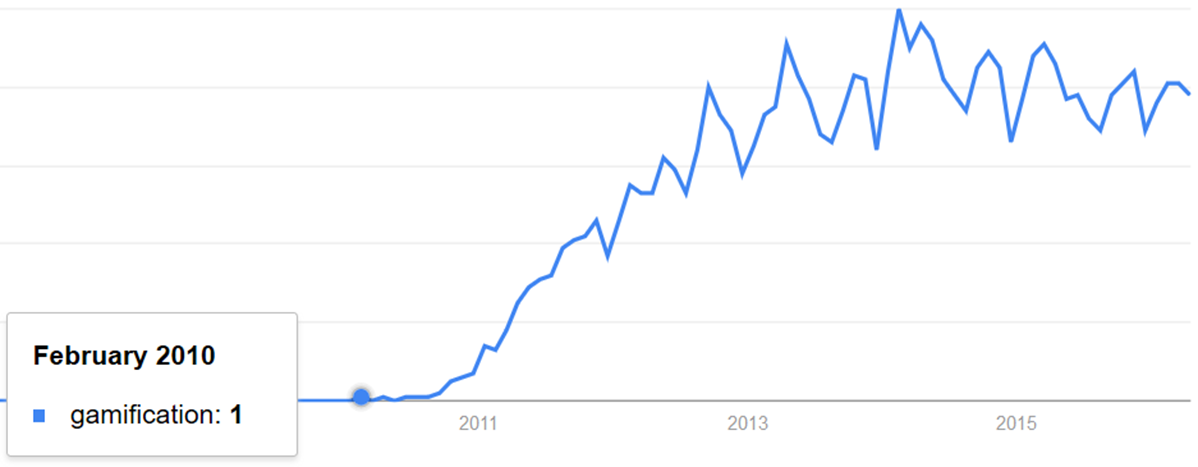
\includegraphics[width=12cm]{gamification-trend}
\caption{"Gamification" on Google Trends per 12 April 2016.}
\label{gamification-trend}
\end{figure}

Real-world examples that show the success of the Gamified Approach are Duolingo\footnote{\url{https://www.duolingo.com/
}} and Re-mission\footnote{\url{http://www.re-mission.net/
}}. Duolingo is a gamification of language learning. It embeds game elements, such as points, levels, and lives, to make language learning more fun. Re-mission is a third person shooting game dedicated to young cancer patients and designed to teach and learn how to deal with cancer. The patients are invited involve in an entertaining game play that will affect their specific behavioral and psychological outcomes toward effective cancer therapy.
      
Through systematic review, Connolly et al. studied the impacts of computer games and serious games regarding engagement and learning in diverse fields. They reported manjority of the studies presented empirical evidence about the positive impacts of computer games and serious games  \cite{connolly2012systematic}. Using the same type of method, Hamari et al. found that according to the most of the reviewed papers, gamification does generate benefits and positive effects \cite{hamari2014does}. Specifically in the field of software engineering, Pedreira el al. also performed  systematic review to investigate the application of gamification in software engineering.  Most of the studies  focus on software development, project management, requirements, and other support areas, but none of them focus on software modelling. They also found less studies reported empirical evidence of their work. They argued that existing studies in the field is quite new, thus more research effort is needed in investigating the impact of gamification in software engineering \cite{Pedreira2015}. 

The report of positive impact of Gamified Approach in various fields encourages us to apply the Gamified Approach in software modelling learning, a subject that seems overlooked for applying gamification. This condition broadens our opportunity to produce novel research contribution regarding the application of gamification in the field of software modelling. Grounded on this background, we then propose our research to investigate and develop software modelling learning games. Since our study is the scope of Model Driven Engineering, we also plan to develop a design framework for the games that will systematically and semi-automatically drives gamification design to produce software modelling learning games. Essentially, our study lies in the intersection between software modelling, learning, and games as depicted in Figure \ref{smlg}. Therefore, we considered to include extensive pedagogical aspect into our study since we are going to address software modelling mainly in it's learning context.    

\begin{figure}[ht]
\centering
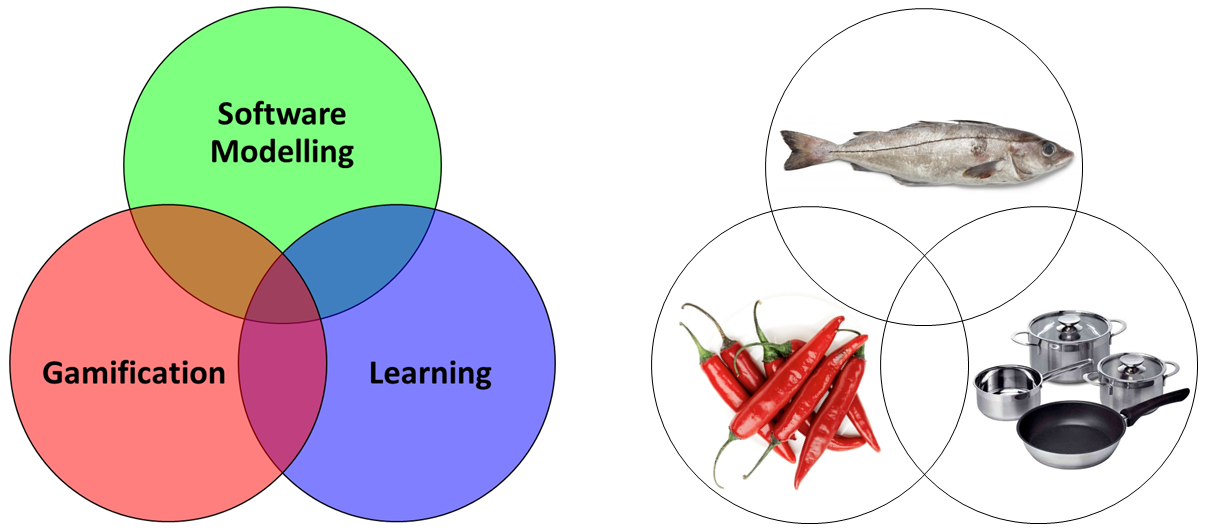
\includegraphics[width=\textwidth]{smlg}
\caption{How to 'Cook' a Gameful Software Modelling Learning?}
\label{smlg}
\end{figure}

This qualifying dissertation is organised as follows. First, we introduce our research in Section 1. We then explain the literature review in Section 2 and propose the research proposal in Section 3. Finally, in Section 4, we end this qualifying dissertation with discussion on our preliminary results. 

\chapter{Field Survey and Review}

Since the research of the gamification of software modelling learning is multidisciplinary study, it is best to organise the literature review categorised by the contributing fields, including the subtopics resulting from the interaction between them. So far, we have identified three major contributing fields, software modelling, ludology, and pedagogy as well (Figure \ref{smlg2}). They will be discussed in the following subsections and a brief review of the research methodology ends this chapter.

\begin{figure}[ht]
\centering
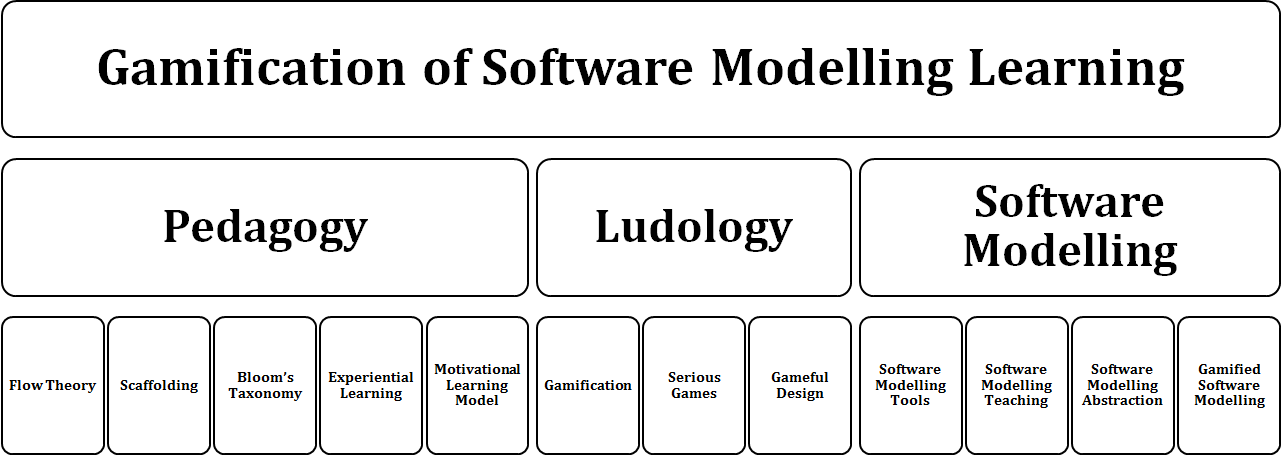
\includegraphics[width=12cm]{smlg2}
\caption{Contributing fields to the gamified software modelling learning.}
\label{smlg2}
\end{figure}

\section{Pedagogy}
\label{Pedagogy}
Designing the gamification of software modelling learning cannot be separated from the field of pedagogy since the core process that will be supported by the gamification is a learning process. Pedagogy has abundance of knowledge and of how we can understand learning processes and from it we could draw principles that will guide the design of software modelling learning games. We have selected several learning models. They are discussed briefly in the following subsections.

\subsection{Csikszentmihalyi's Flow Theory}
Csikszentmihalyi proposed the theory of Flow that states to maintain learner's engagement in an activity, the given challenges and his competence has to be keeped balanced \cite{csikszentmihalyi2014toward}. Once the challenges are too difficult, he will arrive at a state of anxiety that demotivates him and then forces him to withdraw from the activity. On the other side, if the challenges are too easy and his competence is very advance, he will be in the state of boredom which also forces him to withdraw from the activity (Figure \ref{flow-theory}).

\begin{figure}[ht]
\centering
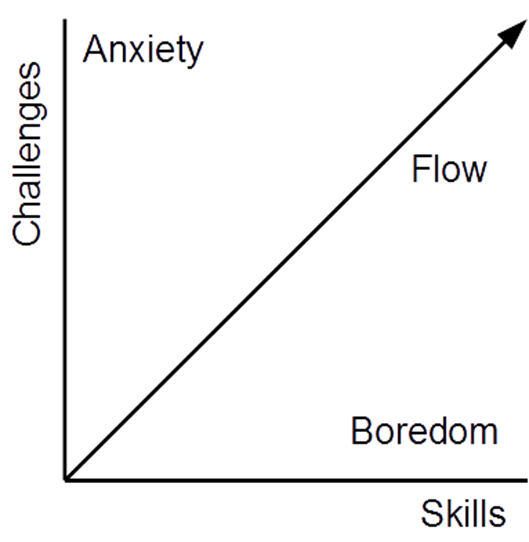
\includegraphics[width=4cm]{flow-theory}
\caption{Csikszentmihalyi's Flow Theory \cite{csikszentmihalyi2014toward}.}
\label{flow-theory}
\end{figure}
    
This theory has been applied in many fields, such as education, training, and games to keep participant engaging with systems. Specifically for games, flow theory influences the design of levels. The given challenges have to  adjusted so they are balance to the skills of players that improve along playing with games. Chen commented well-designed games should bring their players to the flow states, delivering happiness and pleasure \cite{chen2007flow}. In the field of education, Liao also used the theory as a framework to study the emotional and cognitive responses to distance learning systems. He found out that flow theory, the cause and effect of the flow experience, also works  when students use distance learning systems \cite{liao2006flow}. Thus, we see that the theory of Flow is very relevant to our research. We will use the theory to design levels, balancing challenges and learners' competence. 

\subsection{Zone of Proximal Development/Scaffolding}
Zone of Proximal Develoment (ZPD) was proposed by Lev Vygotsky in the context of adolescent development \cite{vygotsky1978mind}. This term was also called Scaffolding by Wood et al. in the context of learning \cite{wood1976role}. The theory states during a learning process, learners have to be reinforced, particularly for knowledge or skills that are very difficult to learn without the support of others, to develop their competence until they are able to acquire the knowledge and skills on their own (Figure \ref{scaffolding}). 

\begin{figure}[ht]
\centering
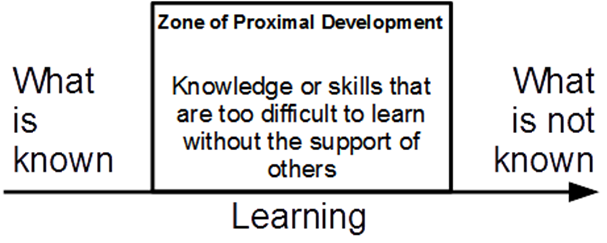
\includegraphics[width=6.5cm]{scaffolding}
\caption{Zone of Proximal Development/Scaffolding \cite{vygotsky1978mind},\cite{wood1976role}.}
\label{scaffolding}
\end{figure}

Kao et al. studied customised scaffolds of an educational game for learning physics \cite{kao2015designing} and Tsai et al. investigated the use of scaffolding aid with importance and use of targeted content knowledge in educational simulation games \cite{tsai2013importance}. Both found proper scaffolding facilitates learning and help learners to have better performance. Since the output of this research is a also a learning game, we decided that the game should also be designed according to scaffolding model. It should present helpers and cues to learners to support them solve problems and grasp important concepts. The scaffolding will be removed gradually as the competence of the learners grows.

\subsection{Revised Bloom's Taxonomy}
Bloom's Taxonomy \cite{krathwohl2002revision} is a framework of cognitive levels for learning process. The framework has been proven very useful for more than 50 years, all over the world, in supporting educators design learning instructions \cite{munzenmaier2013bloom}. It consists of six activities for students in learning, namely remember, understand, apply, analyse, evaluate, and create, and order them according their cognitive load levels with 'remember' at the bottom and 'create' as the activity that require cognitive load most (Figure \ref{bloom}). 

\begin{figure}[ht]
\centering
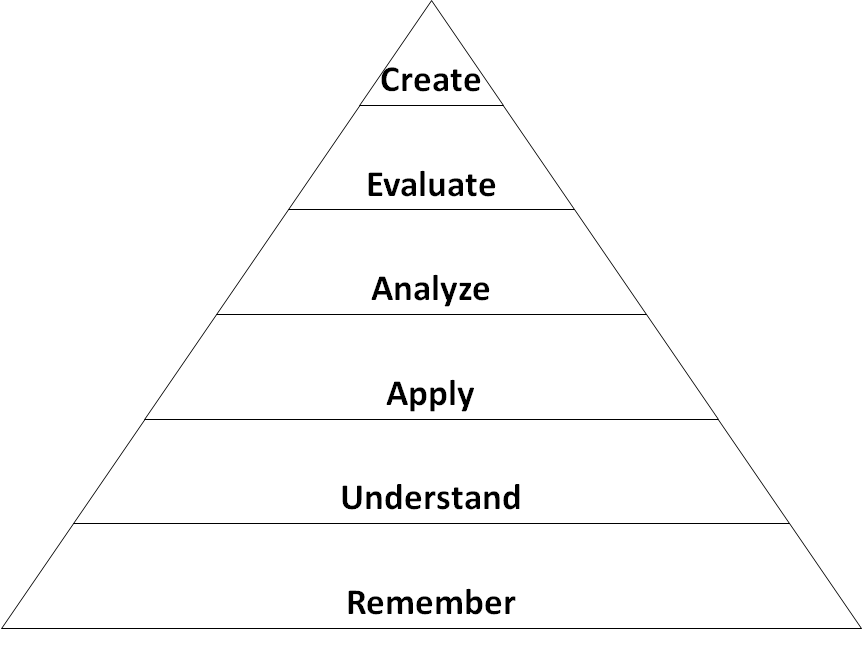
\includegraphics[width=6cm]{bloom}
\caption{Revised Bloom's Taxonomy\cite{krathwohl2002revision}.}
\label{bloom}
\end{figure}

Bloom's taxonomy has been used by other researchers in their studies. Arnab et al. utilised learning activities in the taxonomy to identify and map learning mechanics to learning mechanics to construct Learning Mechanic-Game Mechanics model  for designing Serious Games \cite{arnab2015mapping}. Von Vangenheim et al. \cite{von2013scrumia} also developed an educational game for teaching SCRUM and applied activities in the taxomony as a standard to assess the achievement of their respondents. 

Likewise these two studies, we also identify the usefulness of using the Bloom's Taxonomy activities to design the activities and challenges of our software modelling learning game. We see the potential of the six activities of Bloom's taxonomy are the activities that the learners will perform when playing the game and the nature of cognitive load of each activity could be applied as the challenges of each level. Thus, Bloom's Taxonomy will give us variety of options--activities and challenges--in designing the levels of our game.

\subsection{Kolb's Experiential Learning Model}
Kolb's Experiential Learning Model is a model of teaching and learning through experience and reflection on actions \cite{kolb2014experiential}. It states that knowledge development is a product of experience or iterative search. The model has a cycle consists of four steps: abstraction conceptualisation, active experimentation, concrete experience, and reflective observation (Figure \ref{kolb}). 

\begin{figure}[ht]
\centering
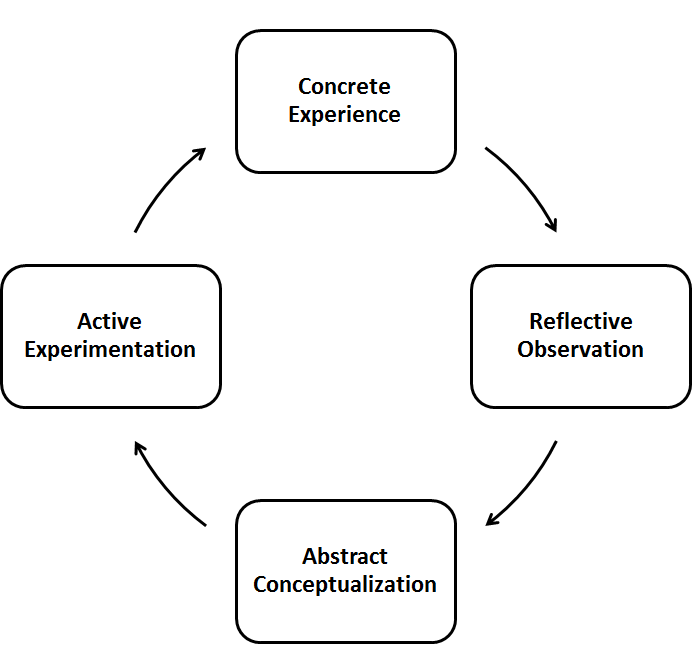
\includegraphics[width=8cm]{kolb}
\caption{Kolb's Experiential Learning Model \cite{kolb2014experiential}.}
\label{kolb}
\end{figure}

As an example, in a case of didactic learning with practicals, learners are firstly taught about the theory. In this step learners perform abstract conceptualisation. They then move to the practicals which they are asked to perform some active experimentation of the theory they got in the class. Through the experimentation they feel the the concrete experience. The results might be to some degree confirm to or disagree with the theory. In the end, through reflective observation, the results are then reconciled with the knowledge they had built based on the theory, whether the knowledge is updated or not. 

A game is a potential tool to realise the experential learning Kolb proposed, since playing games demands learners to actively participate in their course, reflect on their achievements as well as strategies and outcomes, and plan their next actions carefully to improve their performance. As a showcase, Bliemel and Hassan used IT manager-like game as  an experential learning tool and found that the experience developed during playing the game helps learners to connect IT management theories and their applications \cite{bliemel2014game}. Boctor studied the use of a game that facilitates experiential learning to reinforce the learning of nursing material. His respondents found this learning method beneficial and enjoyable to learning \cite{boctor2013active}. 

These studies encourage us to also apply experiential learning into the design of our game so it will allow learners to perform active experimentation and develop their own understanding in software modelling. Kolb's cycle provide us a framework how we should design the activity cycle when learners engage with the game and to help them to connect their knowledge and practice.    
  
\subsection{Keller's ARCS Motivational Learning Model}
Keller's Motivational Model is a set of steps for promoting and maintaining motivation in a learning process \cite{keller2010motivational}. The steps are attention, relevance, confidence, and satisfaction (Figure \ref{keller}). Attention means how to arouse learners to get their attention. Relevance is using  examples and languages familiar to learners. Confidence means establishing and maintaining positive attitude to achieve success or good learning. Satisfaction is to value and reward learners' achievement.   

To maintain the motivation of learners in a process of learning, first, we need to draw the attention of learners using novelty, surprise, aesthetics, or questions. After that, we should explain the relevance of the topic that is about to be explained. We could present the objectives, usefulness, instructions, motives, and contexts. Along the learning process, learners' motivation is maintained by raising the confidence of the learners through presenting their progress, performance, challenge, success, and ability. In the end of the learning process, learners should experience the satisfaction which can be realised by presenting them achievement, enjoyment, rewards, motivation, and feedback.

\begin{figure}[ht]
\centering
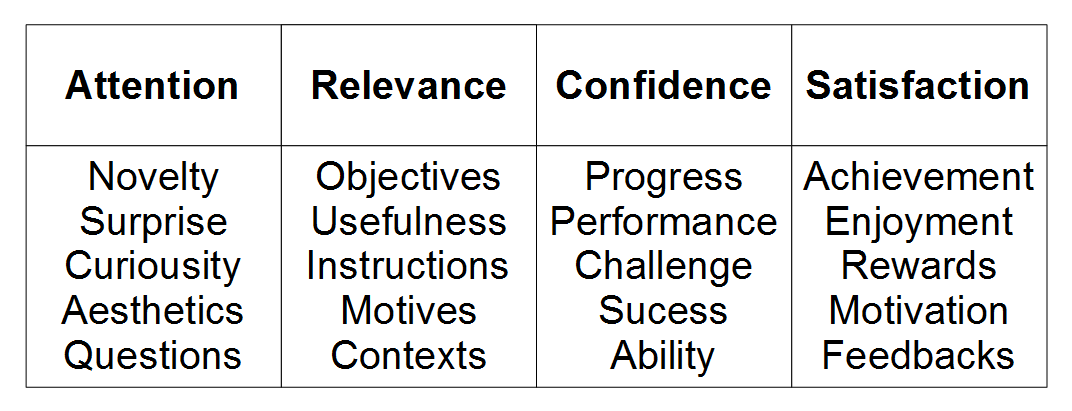
\includegraphics[width=10cm]{keller}
\caption{Keller's Motivational Model \cite{keller2010motivational}.}
\label{keller}
\end{figure}

Throughout their experiment using ARCS model to examine the motivational aspect when learners play digital game-based learning, Huang et al. found that motivational processing (attention, relevance, and confidence) need to be considered when designing DGBL \cite{huang2010sustaining}. Likewise, Derbali and Frasson studied players' motivation during playing a serious game. Using Keller's motivational model and  electroencephalography to measure leaners' motivation, they found out that learning using serious game significantly increases learner motivation \cite{derbali2010players}. Therefore, for the design of our game, we judged Keller's model is useful for designing the flow of a level of a software modelling learning game as it mentions steps that we need to focus to maintain learners' motivation. We will implement the four steps of Keller's model in course of a level.  

\section{Ludology}

\subsection{Serious Games and Gamification}


\subsection{Hunicke's MDA Model}
Hunicke's MDA Model \cite{hunicke2004mda} consists of three steps in designing a game. They are menchanics, dynamics, and aesthetics. Mechanics means the algorithms and data representation used as the backend of the game. Dynamics is runtime behaviour, mechanics, and player inputs and outputs overtime. It is the interaction between players and the game. Aesthetics is player's emotional responses. Design of a  game has to balance challenges and player's skills to keep the player flowing.

\begin{figure}[ht]
\centering
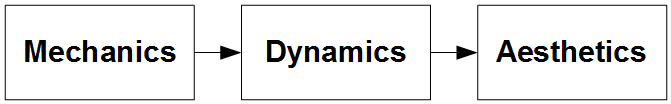
\includegraphics[width=8cm]{mda}
\caption{Hunicke's MDA Model \cite{hunicke2004mda}.}
\label{fig:mda}
\end{figure}

\subsection{Werbach's Gamification Framework}
Werbach and Hunter proposed a Gamification Framework to guide the implementation of a gamification \cite{werbach2012win}. The framework consist of  a prescriptive model of implementing gamification and a structural model of game element hierachy. The prescriptive model consists of 6D implementation steps, which are (1) Define  business objectives. (2) Delineate target behaviours. (3) Describe your players. (4) Devise activity cycles. (5) Don't forget the fun! (6) Deploy the appropriate tools.

The hierarchy consists of three layers, dynamics, mechanics, and components. Dynamics are the big-picture aspects of the gamified system that one needs to consider and manage but which can never directly present in the system. Mechanics are the basic processes that drive the action forward and generate player engagement. Component are the specific instantiations of mechanics and dynamics. 

\begin{figure}[ht]
\centering
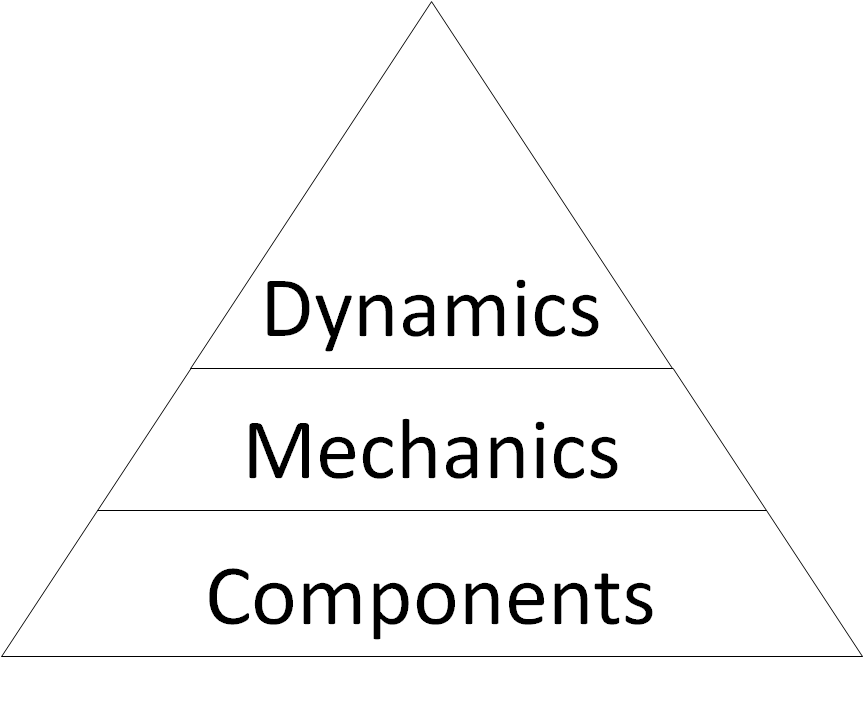
\includegraphics[width=6cm]{werbach}
\caption{Werbach's game element hierarchy \cite{werbach2012win}.}
\label{fig:werbach}
\end{figure}

\subsection{Learning Mechanics-Game Mechanics Model}
Learning Mechanics-Game Mechanics (LMGM) Model consists of 2 sets of mechanics: learning mechanics (LM)  and game menchanics (GM) \cite{arnab2015mapping}. Each mechanics comprises of activities relevant to the aspect that each represents. For examples, modelling, analyse, and discover in LM, and role play, strategy/planning, and selecting/collecting in GM. They act like an inventory which a game designer can select the best mechanics from each mechanics group that fit to a context. The mechanics are then integrated into players' activity cycles.

\begin{figure}[ht]
\centering
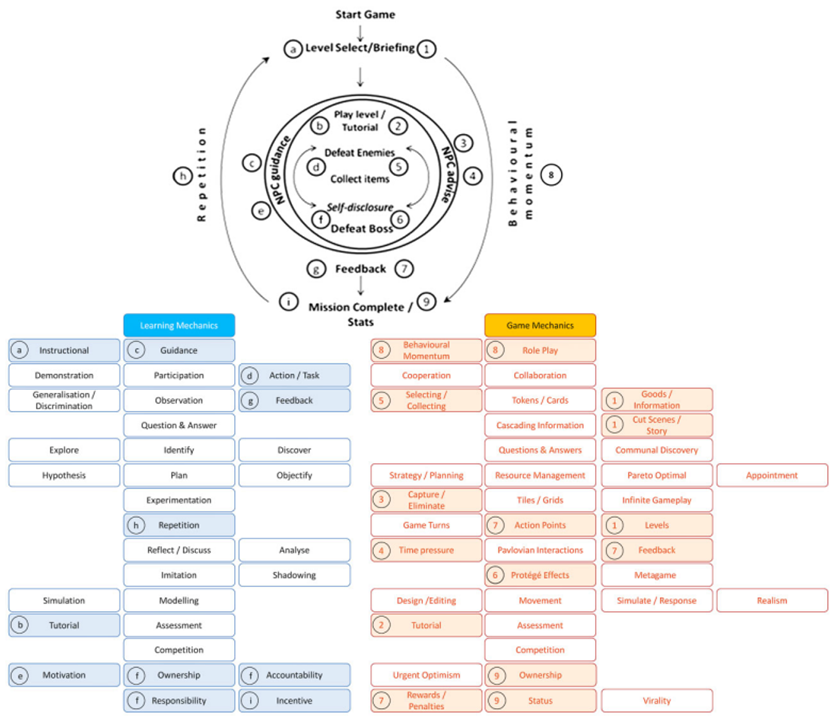
\includegraphics[width=12cm]{lmgm}
\caption{Learning Mechanics-Game Mechanics Model \cite{arnab2015mapping}.}
\label{fig:lmgm}
\end{figure}


\section{Software Modelling}

\subsection{What is Software Modelling?}

concretisation
\begin{figure}[ht]
\centering
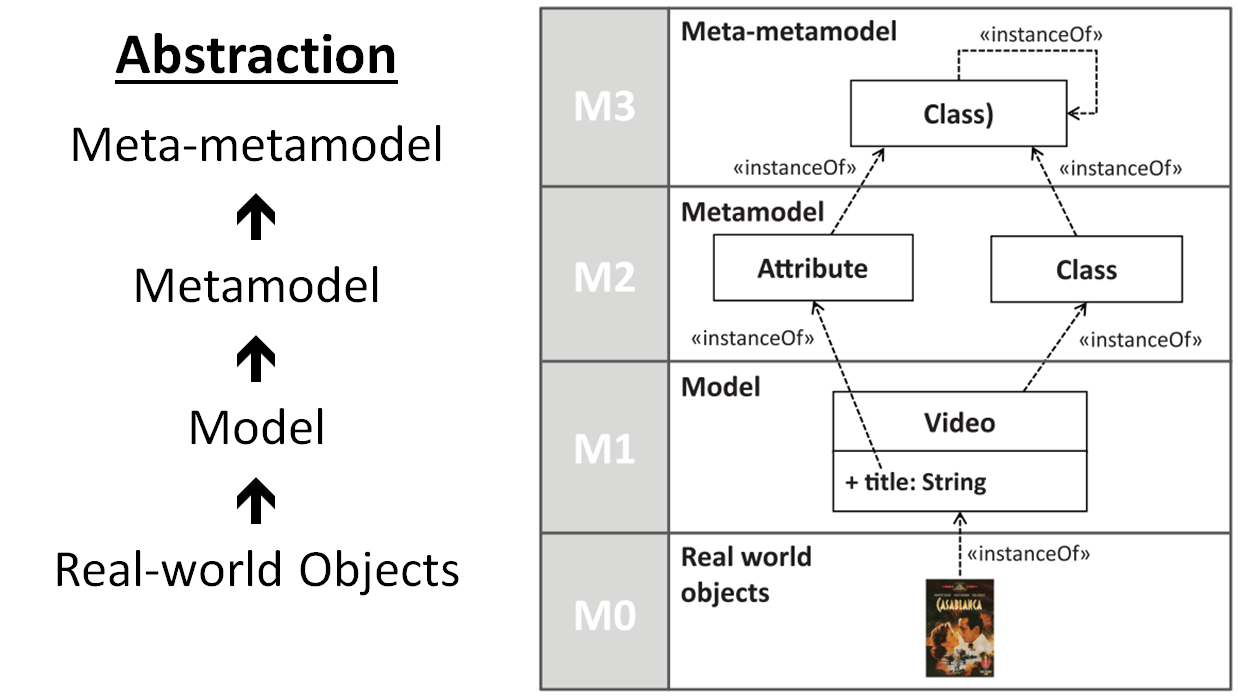
\includegraphics[width=8cm]{abstraction}
\caption{Abstraction in Model-driven Engineering \cite{brambilla2012model}.}
\label{fig:abstraction}
\end{figure}


\begin{figure}[ht]
\centering
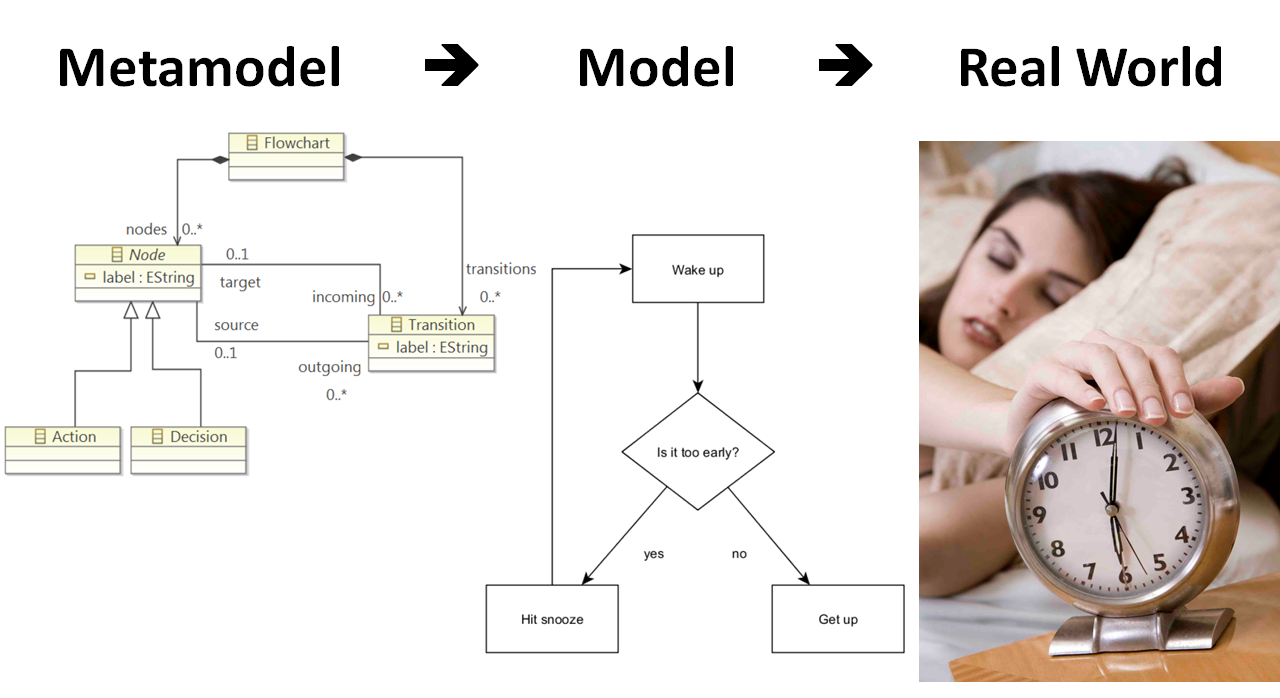
\includegraphics[width=8cm]{concretisation}
\caption{Instantiation in Model-driven Engineering.}
\label{fig:concretisation}
\end{figure}

\subsection{Software Modelling Tools}

\begin{figure}[ht]
\centering
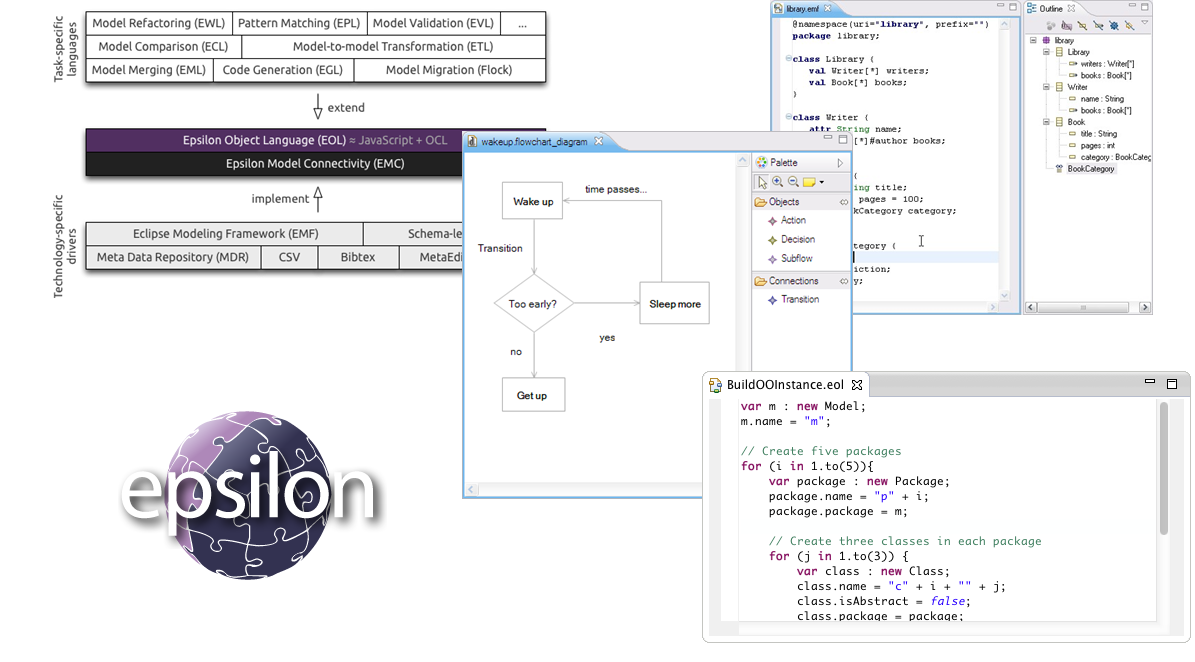
\includegraphics[width=8cm]{epsilon}
\caption{Epsilon is a family of languages and tools for model management\cite{kolovos2015eugenia}.}
\label{fig:epsilon}
\end{figure}

\subsection{Software Modelling Course at the University of York}


\subsection{Software Modelling Teaching}
\label{Software Modelling Teaching}
We have investigated related literatures regarding the teaching and learning of software modelling.  From the literatures, we have identified lessons and categorised them into 3 groups: contents, teaching or learning practices, and tool design. We will take into account the lessons during the design process of our gamified software modelling learning since we want to develop our research upon other existing works thus have stronger foundation.   

\subsubsection{Contents}
Contents mean the software modelling topics and their structures. In teaching software modelling, we need to teach the core, important concepts and their relation with the contexts and applications of the outside world. The contents of software modelling learning should be:
\begin{enumerate}
\item Software modelling definition \cite{borstler2012teaching}.
\item Semantics, syntaxes, notations. Teach modelling foundations, but focus more on semantics, not only syntax \cite{borstler2012teaching}. Improve use of language, not only vocabulary \cite{bezivin2009teaching}.
\item Modelling, metamodelling, and model transformation. Focus on the core, important concepts: modelling, meta-modelling, and model transformation. Teach modelling that comprise the following topics: formal and informal models, partial and complete models, distinction between models and programs \cite{bezivin2009teaching}. Meta-modelling is given a larger portion than modelling since a model might conforms to more than one meta-mode \cite{ober2007teaching}.
\item Software modelling is engineering. Teach the engineering aspects of software modelling: understanding a domain, planning and resourcing, documentation, quality, formality, validity, optimisation \cite{paige2014bad}.
\item Contexts and practices/applications in various domains \cite{paige2014bad}. Teach the application of software modelling in various domains, success stories, code generations, model discovery, and model-driven interoperability. Make the model executable. Still the power of execution makes it much easier to understand the model \cite{bezivin2009teaching}. Convey the practical applications of modelling \cite{borstler2012teaching}.
\end{enumerate}


\subsubsection{Teaching and Learning Practices}
Teaching and learning practices are the principles, values, and methods in teaching or learning software modelling. The followings are them:
\begin{enumerate}
\item Modelling is the process to think abstractly about systems. Therefore, we teach modelling to make students understand the value of abstraction \cite{bezivin2009teaching}. Successful application of Model-Driven Software Development requires skills in abstract modelling \cite{whittle2013industrial}.
\item Teach with prerequisites \cite{paige2014bad}. Student should have a good programming background \cite{bezivin2009teaching} or has to know a little about OOP \cite{Akayama2013}.
\item Encourage students to produce "good" models, and measure the "quality". One way is to use tools \cite{Akayama2013}.
\item Learn modelling as early as possible \cite{Akayama2013}, \cite{borstler2012teaching}. Teach modelling together with programming (Börstler et al., 2012). Modelling should be developed alongside programming \cite{bezivin2009teaching}.
\item Problem-solving first, modelling language specification and modelling tools get in the way \cite{paige2014bad}.
\item Provide solutions, not answers \cite{paige2014bad}.
\item Teach modelling language broadly, not deeply \cite{paige2014bad}, and throughoutly \cite{borstler2012teaching}). Students need to experience the whole cycle of modelling in a software engineering project so they learn to decide which development process is more appropriate \cite{Akayama2013}.
\item Refer to other disciplines or other aspects related to software modelling \cite{paige2014bad}.
\item Even though code generation is essential to understand modelling \cite{liebel2015ready},  teach other applications (benefits) of software modelling at first. Code generation comes later \cite{paige2014bad}.
\item Be careful when using analogies and physical decomposition, since they might not reflect the complexity of the system; one component might have a cross-cutting effect to other layers of the system \cite{paige2014bad}. 
\item It is good to teach modelling with a standard language, such as UML \cite{bezivin2009teaching}, but teach modelling and meta-modelling using other modelling languages as well, not just UML. Software modelling is not a UML modelling course \cite{paige2014bad}. A significant number of successful Model-driven Software Development companies build their own modeling languages and generators, suggesting a re-orientation of education away from UML notation to fundamental modeling principles \cite{whittle2013industrial}.
\item Choose a playful domain or fun problems, not serious domain \cite{paige2014bad}.
\end{enumerate}

\subsubsection{Tool Design}
Tools design are the principles in designing software modelling tools. Since we are going to develop a tool that can support learners to learn software modelling, lessons in this category will have important in guiding the design of our tool. 
\begin{enumerate}
\item Learning modelling tools is not trivial (Paige et al., 2014). 
\item Build knowledge and skills incrementally \cite{lethbridge2014teaching}.
\item Use papers, tools designed for pedagogy, or use mainstream tools \cite{Akayama2013}.
\item The usage of modelling tools is not important in the beginning, but later when modelling task becomes larger \cite{bezivin2009teaching}.
\item A good experience with the tool has a positive influence on the students’ view of UML and modelling in general \cite{liebel2015ready}.
\item Support for tool usage greatly affects student satisfaction. Provide Tool Expert and carefully design the instructions if you are using Industry Modelling Tool \cite{liebel2015ready}. For an example, Papyrus is suitable for a classroom environment if given the right level of support \cite{liebel2015ready}.
\item Give positive reinforcement to learners \cite{lethbridge2014teaching}.
\item The tools gives maximum opportunities for learning \cite{lethbridge2014teaching}.
\item The tool convinces learners of the value of what they learn \cite{lethbridge2014teaching}.
\item Focus on high usability \cite{lethbridge2014teaching}.
\item The tool is inexpensive \cite{lethbridge2014teaching}.
\end{enumerate}


\subsection{Abstraction in Software Modelling Learning}
Following the last discussion, modelling and meta-modelling, and additionally model management, are the potential concepts that will be taught in the game. All the three concepts requires adequate abstraction skill; a skill that has a fundamental role in Computer Science and Software Engineering (Engels, Hausmann, Lohmann, \& Sauer, 2006; Hazzan, 2008; Kramer \& Hazzan, 2006). 
There are some available strategies in teaching abstraction. Familiarity, Similarity, Reification, Application. This strategy is proposed by White and Mitchelmore in the Math education (White \& Mitchelmore, 2010). They argued that abstraction should be developed from empirical experience, move up to abstraction, and concreting the abstraction through application. Similarly, based on their experience teaching UML, Engels et al. (Engels et al., 2006) approached abstraction through modelling according to this steps: real-word objects, object diagrams, class diagrams. The real-world objects can be described by videos or may be substituted by textual explanation, animations, or pictures. Hazzan (Hazzan, 2008) proposed three methods in teaching abstraction. First, illustrate. Lecturer uses abstraction-related words or statements in teaching. Second, reflect. For an example, lecturer and students question the impact of using certain level of abstraction or not using abstraction at all. Third, practice. Students must practice and reflect on what he do.

There are two approaches of learning software modelling which a learner may perform them simultaneously: rational approach and intuitive approach (Bobkowska, 2014). Usually at the beginning of modelling process, one uses his existing knowledge and logical reasoning to understand and develop software models, and sometimes preceded with empirical activities. However, there are situations in software modelling when his existing knowledge and methodology-based, logical reasoning are not enough to make him understand or to develop a software model. Thus, make him relies on his own intuition or both approaches interplay in dealing with complex, difficult modelling. In line with Bobkowska's statement, in building a model on the correct level of abstraction, one needs a certain intuition and skill which cannot be gain through lectures but have to be experienced through exercises (Engels et al., 2006).

\subsection{Gamified Software Modelling}
Most of the gamification studies available are dominantly relates to software engineering in a larger context or other aspects of software engineering, such as software implementation and project management, rather than software modelling in particular \cite{Pedreira2015}. Several studies that apply gamification specifically for software modelling are the works of Stikkolorum et al. \cite{Stikkolorum2014}, Ionita et al. \cite{Ionita2015}, Groenewegen et al. \cite{Groenewegen2010}, and Richardsen \cite{Richardsen2014}. These works are selected because they develop artefacts based on gamification approach, apply them to software modelling, and validate the results.

\subsubsection{Puzzle Game to Teach Software Design Principles}
Stikkolorum et al. \cite{Stikkolorum2014} developed a game that is intended to teach software design principles, such as cohesion, coupling, information hiding, and modularity in software design.They tried to look for a solution that provides balance between coupling and cohesion by using the toolbox to draw classes, methods, attributes, and relationships between them. They applied game elements like puzzle game, game levels, visual and audio feedbacks, progress indicator, level unlocking, choice of path, multiple solutions, scoring. For the pedagogical aspect, they mentioned Bloom’s taxonomy in their work. However, they did not explain how they integrated the taxonomy into their work. After using their game, users started to talk regarding classes, methods, and associations instead of boxes, blocks, and lines, indication unconscious learning. The challenges of their work were on determining scores because there are more than one solutions for a problem. To determine coupling, they used Coupling Between Classes (CBO). Cohesion was measured by comparing all items—attributes, methods, class name—in a class that have similar keywords. Information hiding and modularity is evaluated using general design patterns. They validate their design by conducting user test and utilise the 'think aloud' method—asking users to tell their thoughts while using the game. 


\subsubsection{Explorable Board-game to Understand and Validate Enterprise Architecture}
Groenewegen et al. \cite{Groenewegen2010} applied gamification to improve stakeholders' understanding of their enterprise architecture models as well as to validate them.
They employ exploring the model step by step, element by element according to the given rules technique which can provides a player a progressive user experience. Therefore, it can improve user understanding. The game proposed is more playable, more freedom to try and explore, and no explicit rewards given. For the game elements, they utilise cards, explorable board-game, and rules. 
Regardless of their claim that users can understand the model better rather than by merely looking at the model so they can give argument whether the model is valid or not based on their existing knowledge, they never clearly discussed the pedagogical aspect of their work. The challenges that they experienced during the implementation of their are preparing the game by translating implicit knowledge to explicit knowledge of the model—a gap of knowledge between the modeller and the reader, which domain knowledge is required. Lack of domain knowledge will make the model less understandable and the user cannot validate the model. For validation, they tested their work to seven respondents and then interviewing them. 

\subsubsection{Familiar Tangible Model to Model Information Security}
In the domain of information security modelling, Ionita et al.\cite{Ionita2015} developed a socio-technical modelling language (TREsPASS) and map them toward tangible representation. Mapping the socio-technical modelling language to the tangible model is the most challenging part of their work. The tangible representations will increase the familiarity and understandability of models, which will increase awareness, involvement, and learnability. For the game elements, they utilise familiar, tangible representation, such as Lego characters, board-game metaphor, rules. They also discussed the pedagogical aspect of their design which is based on the theory of constructionvism, cognitive load, and cognitive fit. Moreover, based on their experiment, they reported that experimental group performs better than the control group in learnability, efficiency, correctness, and satisfaction. Likewise, based on interview with experts and professionals, the respondents argued that the tangible model might be useful for less technical domain experts and different types of stakeholders to be more participative and contributive in the early stages of architecture modelling.

\subsubsection{Arranging UML Activity Diagram to Control the Behavior of a Game}
In the context of activity diagram learning, Richardsen  \cite{Richardsen2014} developed a game which it's behaviours are controlled through arranging UML activity diagram. Throughout his research, he found challenge that controlling game from activity diagram in Reactive Block Environment (Eclipse based) is difficult since Eclipse is difficult for a first-time user. For validation, he conducted user testing with three users. Think Aloud method was used for observation. After that, questionnaires were given and an interview was conducted. he found out There was no significant different between the traditional interactive tutorial and the game-like tutorial on their performances. However, the game-like tutorial was more engaging. For the validation of his work, he did not mention any explicit pedagogical aspect.\\

Based on the previous four related works, we concluded that different concepts of software modelling were addressed. However, no use of game elements that addresses abstraction regarding modelling, meta-modelling, and model transformation in particular, which mean there is an opportunity for research on that area. We also found that different specific concepts were addressed with different approaches and game elements which also challenge us to develop a more generic design in addressing software modelling learning problem. The good news is all of the works reported that the use of game and game elements has positive effect in motivating and engaging users in varying degree. Furthermore, every study has their own challenges which are a good thing to be aware of when carrying our research. The drawbacks of other works are, first, most of the them did not consider seriously about pedagogical aspect of their solution and, second,in general, their validation was weak regarding sample size and lack discussion of internal validity.




\section{Research Methodology}
The software modelling learning game design framework will be derived deductively mainly from existing related theories and research works that come from the fields of education, games, and software modelling. The resulting framework will be tested in several case studies for validation and the test results will be inputs to revise the framework. Since the outputs of the research will be design artefacts, Design Science Research Methodology \cite{peffers2007design} is selected as the research methods as it provides a comprehensive conceptual framework and activity guidelines for understanding, developing, executing, and evaluating design artefacts. We also implements Deterding's Gameful Design Steps \cite{deterding2015lens} to guide the design of the gameful aspect of the the product.

\subsection{Design Science Research Methodology}
We will employ Design Science Research Methodology \cite{peffers2007design} as the methodology to carry out the research. DSRM is selected since it provides a comprehensive conceptual framework consists of activity guidelines for understanding, developing, executing, and evaluating design artefacts. Oher reason is that it positions itself at the top level of abstraction without going into much detail of how to perform each activities, we can freely choose other more concrete research methods to carry out the activities. For examples, we can conduct literature reviews, surveys, or expert interviews to determine research problems, motivations, solutions, and objectives as well as controlled experiments to measure and evaluate the effectiveness of the artefacts. 

\begin{figure}[ht]
\centering
\frame{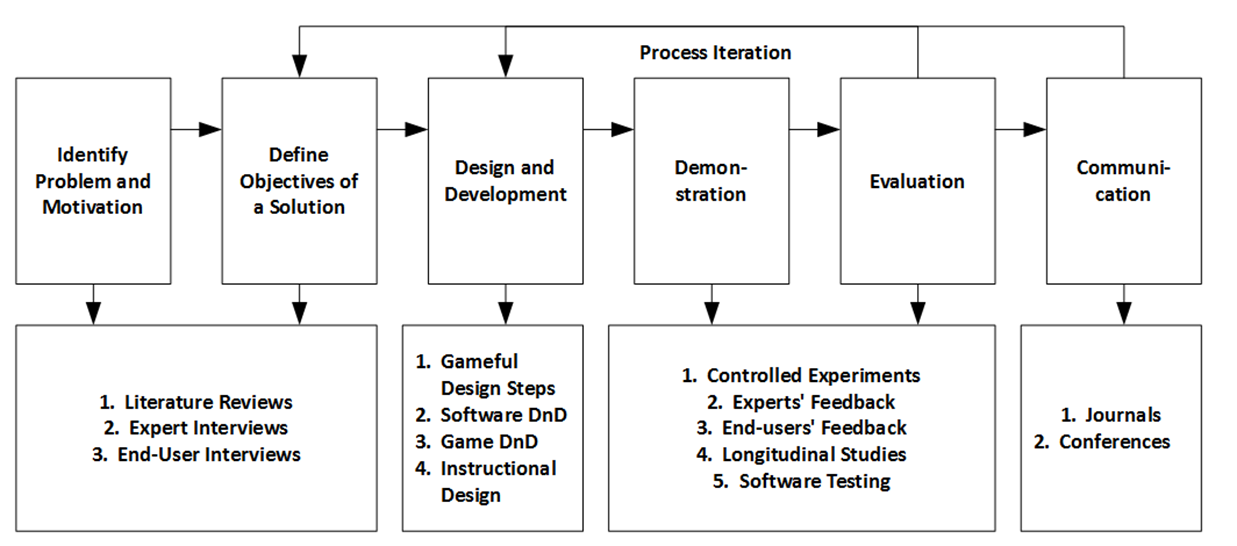
\includegraphics[width=\textwidth]{dsrm}}
\caption{Design Science Research Methodology. Adapted from Peffer et al. \cite{peffers2007design}.}
\label{fig:003}
\end{figure}

\textbf{Identify Problem and Motivation}. This research will use literature review, suggestions from experts, and surveys to identify research problems and motivations a well as to determine the solution and its objectives.

Based on the literature review, the best guesses that we have made so far regarding the challenges that student has to deal with when learning software modelling are abstracting (choosing the most relevant elements, ignoring the irrelevant ones, and determining the relationships between elements), diagramming (translating the abstraction into visual elements), and determining the algorithmic strategies (programming in the context of model management). Other challenges are no fun (the presentation of the software modelling course is not interesting) and the heavy cognitive loads when dealing with abstract objects. However, the guesses have to be confirmed yet through surveys, drawing information from students of software modelling courses in order for our problem identification to be more accurate.

As we could view the challenges as problems, this research then chooses the problem-centred initiation as its entry point since those challenges hinder learners in learning software modelling.  Grounded on the identified problems, we could decide that there is a necessity to build a tool that can support software modelling students to develop their abstraction, diagramming, and algorithmic strategy skills in a more motivating and engaging way. 

\textbf{Define Objectives of a Solution}. Based on the identified problems and motivations, we have defined our solution that is embedding gamification in the process of software modelling learning, which is expressed by the use of an artefact specifically designed with gamification and pedagogy in mind. The research objectives and outcomes are defined in section 3.2 and 3.3.

\textbf{Design and Development}. This research will employ gameful design method (Deterding, 2015) to design and develop the gamification and agile software development method to design and develop the artefact. The design and development activities are part of the iterative cycles and the products of the activities will be refined as required based the results generated from the evaluation activity.

\textbf{Demonstration and Evaluation}. The resulting artefact will be demonstrated and evaluated by applying it to several courses of software modelling. Moreover, the evaluation results will be used as feedbacks to improve the quality of artefacts and as a ground to judge the research findings.  Demonstration and evaluation activities are parts of the iterative cycles and will be performed again as required. 

\textbf{Communication}. Significant findings will be published in an academic conferences or journals for dissemination and evaluation by the related research communities.


 
\subsection{Gameful Design Method}
Deterding proposed a gameful design method that consists of gameful design steps, a set of design lenses, and skill atoms \cite{deterding2015lens}. Gameful design method is a prescriptive guideline to implement gamification that comprises five phases: strategy, research, synthesis, ideation, and ideation. 

In strategy phase, stakeholder define outcome metrics, target users, context, and activities as well as constraints and requirements. In the next phase, research phase, user activities behaviour chains, user needs, motivations, and hurdles as well as how game design fits with them are identified and defined. After that, in the synthesis phase, triplets or a combination of activity, challenges,  and motivation is defined,including defining skill atoms. Furthermore, in the ideation phase, to generate ideas of the gamification design, brainstorming with innovation stems are conducted. Design lenses are used to help view the triplets from the perspective of game elements. After some ideas are generated, those ideas are prioritised. The prioritised ideas are then translated into storyboards to make them more visible. After that, the ideas are evaluated and refined based on results of the evaluation. In the last phase, a prototype is developed iteratively. This includes the activities of playtesting, analysing, building, and generating new ideas.  

\begin{figure}[ht]
\centering
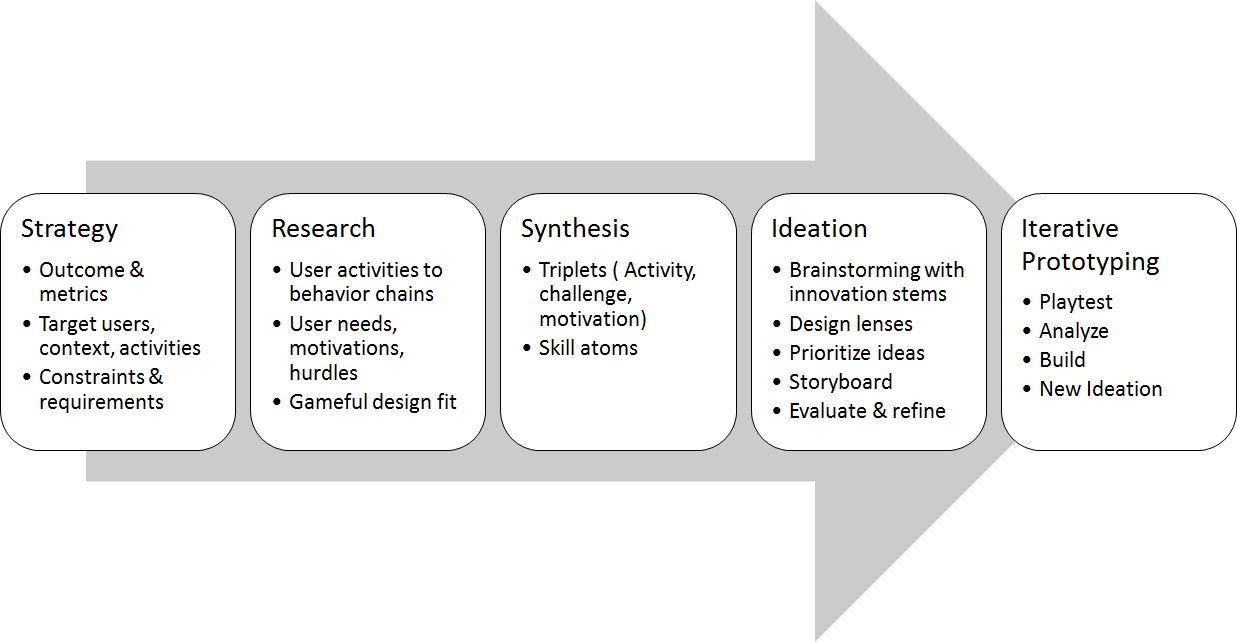
\includegraphics[width=8cm]{gameful-steps}
\caption{Deterding's gameful design steps \cite{deterding2015lens}.}
\label{fig:gameful-steps}
\end{figure}

Design lenses is a combination of an easy-to-remember name, a short statement of a design principle, and a set of focusing questions that helps designer to view activities, motivation, and challenges from the perspective of the lenses. Design lenses are derived from game elements, so in short, viewing using design lenses means learning to view in the perspective of game elements. Deterding's Design Lenses comes has four categories lenses: challenge, goal and motivation, action and object, and feedback, and each category comes with pre-existing lenses.

\begin{figure}[ht]
\centering
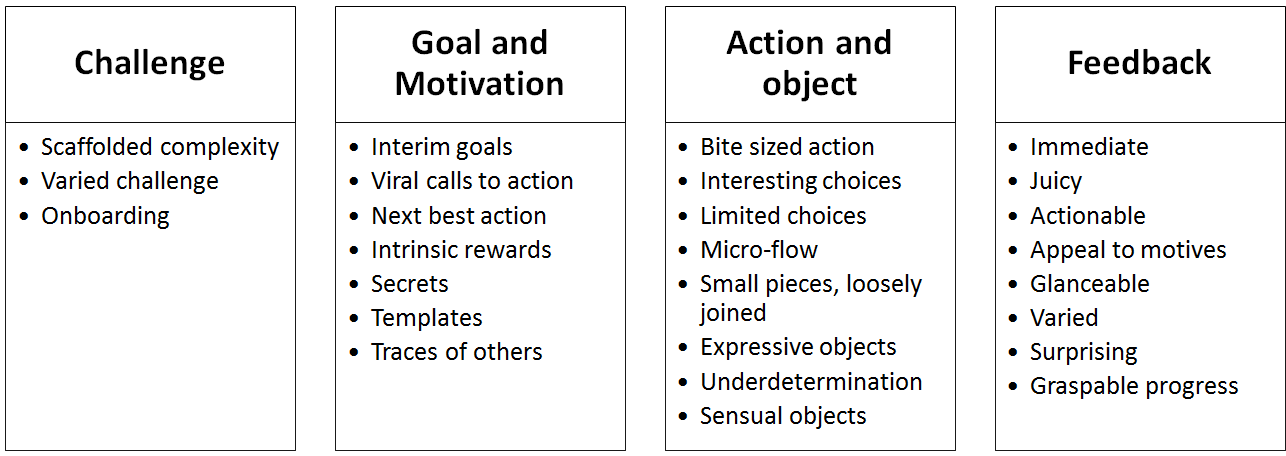
\includegraphics[width=8cm]{lenses}
\caption{Deterding's design lenses \cite{deterding2015lens}.}
\label{fig:lenses}
\end{figure}


A skill atom describes a feedback loop between user and system that is organized around a central challenge or skill: A user takes an action, which forms an input into the system’s rule engine that determines state changes of its tokens, which get put out as feedback to the user, which she integrates into her mental model of the system. Through repeated interaction—multiple run-throughs of the atom—the user masters its skill: training hand–eye coordination, understanding the rules, and so on.

\begin{figure}[ht]
\centering
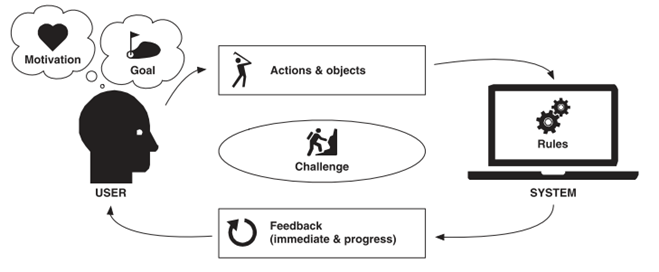
\includegraphics[width=8cm]{skill-atoms}
\caption{Deterding's skill atoms \cite{deterding2015lens}.}
\label{fig:skill-atoms}
\end{figure}

\subsection{Evaluation}
We wish to evaluate (1) the effectiveness of the modelling games discussed above and (2) the productivity and maintainability benefits of the modelling game design framework. For the effectiveness evaluation, controlled experiments will be used. The participants, software modelling students, will be divided into two groups, a control group and an experimental group. The control group will learn software modelling using traditional methods while the experimental group will learn with support from the games. Then, their performance of the two groups will be measured by their ability to solve a set of related modelling problems. 

For the evaluation of the modelling game design framework, the participants will be software modelling tutors; they will be devided into two groups, one that will develop games \emph{with} the framework and one \emph{without} the frameworks (i.e. using existing web technologies). They will be asked to elaborate their games into their teaching instructions and use them in their teaching. The comparison will be on their productivity and the maintainability of their games. To evaluate the generality of the results of both evaluation processes, conducting experiments in different years and countries is also considered.

Additionally, surveying with questionnaires or interviews might be conducted to investigate the underlying variables or processes. Structural equation modelling \cite{hair2016primer} is also an option if measuring the effects of the identified underlying variables is required. An alternative method for understanding of the underlying variables and processes is through investigating the games' event logs using data mining or machine learning techniques.


\chapter{Proposal}
Grounded on the literature review in Chapter 2, we base our research in these premises. First, learning software modelling is not a trivial task as it requires abstraction skills and demands high cognitive loads to deal with abstract objects and operations. Second, regardless gamification design is still an ongoing challenge \cite{Deterding2013}, it is an opportunity for research that up today there is still no work in the gamification of learning that addresses the core concepts of software modelling—modelling, metamodelling, and model transformation. Third, there is still no gamification design framework that guide the integration of game specific domain into software modelling learning. Fourth, opportunity to 

\section{Research Questions}
The main research question proposed by this research is "How can gamification improve software modelling learning?" In order to support answering the main research question, following sub research questions need to be investigated:
\begin{enumerate}
\item Which processes, aspects, principles, or components of software modelling and their teaching and learning practices would benefit from gamification?
\item What types of game elements and in what roles can deliver software modelling learning best? 
\item What kind of orchestrating framework is needed to design the interaction between software modelling and game elements to achieve software modelling gamification?
\item To what extent does gamification of software modelling improve learners' motivation, engagement, and performance?
\item To what extent do software modelling tutors benefit from software modelling game design framework?
\end{enumerate}

\section{Aim and Objectives}
In order to answer the research questions, following aim and objectives should be met. The main aim of this research is to investigate and develop a software modelling game design framework that systematically and semi-automatically drives gamification design to produce software modelling learning games. More precisely, this research aims to meet the following research objectives that are derived from the main research aim:

\begin{enumerate}
\item Perform a literature review and surveys to identify research problems, questions, and objectives as well as necessary information to carry out the selected research methods and to develop an early version of the conceptual framework and artefact as the instantiation of the framework. 
\item Develop a conceptual framework of how to design gamification of software modelling learning based on the literature review and the survey. The framework will be iteratively updated according to the results obtained from the experiments. 
\item Develop a software artefact as the instantiation of the conceptual framework to produce a gamification of software modelling learning. The gamification will be tested to respondents for evaluation and to obtain feedbacks for iterative improvement. 
\item Perform controlled experiments to measure the significance of the sofware modelling learning game in improving learning performance compared to the traditional method.
\item Perform controlled experiments to measure the productivity and maintenabilty of software modelling learning design framework in supporting tutors design and develop gamified software modelling learning. 
\end{enumerate}

\section{Research Outputs}
The potential research outputs of this research are:
\begin{enumerate}
\item Artefact. The software/application of gamification of software modelling learning.
\item Modelling Artefact. A tool for modelling the application of the gamification of software modelling learning.
\item Significance. Controlled experiments, learning outcome comparison between the gamified version and the traditional one.
\item Software Modelling Design Framework. Conceptual and software framework to perform gamification of software modelling learning.
\item Understanding. A model that explains how gamification of software modelling learning works.
This could be achieved through Learning and Game Analytics and Structural Equation Modelling studies.
\item Case Study. Report the application of theories, models, and methods used in this research.
\end{enumerate}

\chapter{Preliminary Results}

\section{Preliminary Survey}
\label{Preliminary Survey}
In this research, we have conducted our preliminary survey. The survey was executed to identify learners' needs, motivations, and hurdles according to the Research phase of the Deterding's gameful steps. This is also inline to the Design Science Research Methodology, which in the first activity we need to identify the problem and motivation so we can define objectives of a solution accurately in the second activity. 

We have distributed online questionnaires to our respondents, students of Model Driven Engineering (MoDE) 2015/2016 module. The students were in their Software Engineering master programme at the University of York. From 21 students, only 4 completed the questionnaires. Their responses can be found in Appendix \autoref{chap:Preliminary Survey Data}.

\textbf{Results}. In order to identify the learners' needs, we asked our respondents question 1 and question 2. Question 1 aims to identify students' expectation before starting the module, while question 2 asked to identify what the students found important after taking the module. Based on the responses, the reasons why the students took MoDE module because they want to increase their knowledge on MDE, posses new advance skills or abilities, and improve their literation of MDE tools. After completing the module, the students valued that the most important lessons were getting new knowledge--domain modelling, metamodel, abstract syntax, abstract thinking, model validation, and the application of models--and skills--generating code, creating DSL, and improving their tool skills.   

We also asked the students question 3, 4, and 5 to identify their motivation in taking MoDE module and learning Model Driven Engineering.  Question 3 asked about the reasons behind their decision taking MoDE module. Two students stated that they took them module because it is compulsory, but the rest of the students said that they took the module because MDE is an advance topic and they wanted to see its applicability in industry and whether it will improve their ability--knowledge and skills. 

Question 4 asked the students about what would motivate them more to learn Model Driven Engineering (MDE). The students gave feedback that they would be more motivated if they could perceive the advantages of MDE: efficiency and effectiveness it could give, the benefits of its application in the organization or real world examples, and its genericity--MDE application in languages other than Java or models other than UML/EMF.

We then asked question 5 which asked the students the most basic, underlying motives that make them commit to learn MDE. Substantially, they answered that their main motivation is to gain new ability--knowledge and skills, such as ability to make abstraction, advance skills that applicable in industry, and knowledge of reallife examples and applications of different models taught in MDE. Nevertheless, passing MoDE module, a pragmatical motives, still part of the whole motivation.  

In question 6 and 7, we asked the students about the interesting challenges that they faced during MoDE module. They mentioned abstract thinking and model management activities such as defining metamodel, validating model, and how to best model a system--satisfying the model's metamodel and validation so the model could be easily queried and transformed). To overcome the challenges, what they did are performing trial-and-error method or experimenting the problems, try many other examples, and completing all the practicals. We summarised all of these efforts as activities to build 'experience'.

We also asked them question 8 and 9 about the non-interesting challenges, extraneous challenges that are not relevant to the core activities of modelling.  They mentioned these activities: dealing with very specific technical concepts/words that only belong to specific products, focusing too much on how to use tools in other words using very tedious tools or less information on how to use the tools, and judging the quality of a model since there was no explanation of how good of bad the model was. To deal with the the uninteresting challenges, they just ignore them, seeking information and solutions from internet, lecturers, assistants, and discussion groups, and redid building the solutions from the beginning when they had certain problems using the tools.

\textbf{Discussion}. There are few takeaways from the preliminary interview in terms of students' needs, motivations, and challenges, that can be implemented into the design of a gamified software modelling learning. \textit{First}, the need of the students to learn MDE is to gain new advance abilities--knowledge and skills--that are applicable in industry, which, if broken drown, they comprise of model management activities (abstract thinking, modelling, metamodelling, model transformation, validation, and application) and tool literacy. 

\textit{Second}, the the motivations of the students to learn MDE are, regardless their view on MoDE module as a compulsary module in their programme, they were aware that their motivation should be on satisfying their need in gaining advance knowledge and skills in MDE as mentioned previously, and they would me more motivated if they could perceive the advantages and applicability of MDE, thus showing students the benefits and applications of MDE is very important in increasing their motivation.

\textit{Third}, they mentioned model management activities (abstract thinking, model validation, metamodelling, etc.) as the interesting challenges. To overcome the challenges, they did trial-and-error method to gain more experience in overcoming the challenges. This is in line to experiential learning which states learning is at it's best through experiencing \cite{kolb2014experiential}. The main concern of gameful design is to reduce the cost of  performing such activities so learners could focus on the core activities without hassles. This could be done by dividing the activities into smaller activity chunks and removing the extraneous, unrelated activities \cite{deterding2015lens}. 

The extraneous, unrelated activities were identified by asking question 8 and 9, which was to identify the uninteresting challenges. Most of the complains were on the tools which were tedious to use. They also argued that there was no need to learn the detailed technical concepts or terms that were only specific to certain products. To overcome the uninteresting challenges, the students preferred to seek information and solutions from on internet, lecturers, and discussion groups. Thus, it is very important to provide comprehensive documentations and supports of the tools used in a learning activity  \cite{liebel2015ready}. 

\begin{table}[ht]
\caption{Requirements derived from the preliminary survey (section \ref{Preliminary Survey}).}
\label{table:preliminary-survey}
\begin{center}
\begin{tabular}{ p{2cm}p{1cm}p{10cm} } 
\hline
Category & Code & Requirements from Preliminary Survey \\
\hline
\multirow{1}{2cm}{Needs} 
& RS01 & Teach them knowledge and skills that are applicable in industry: model management (abstract thinking, modelling, metamodelling, model transformation, validation, and application) and tool literacy. \\ 
\hline
\multirow{1}{2cm}{Motivations}
& RS02 & Promote gaining advance knowledge and skills in MDE. \\ 
& RS03 & Promote the benefits and applications of MDE. \\ 
\hline
\multirow{1}{2cm}{Interesting Challenges}
& RS04 & Challenge with model management activities (abstract thinking, model validation, metamodelling, etc.). \\ 
& RS05 & Scaffold the learning process to support learners gaining their experience (for an example, dividing the activities into smaller activity chunks). \\ 
\hline
\multirow{1}{2cm}{Un-interesting Challenges}
& RS06 & Increase the usability of the tool being used. \\ 
& RS07 & No need to learn the detailed technical terms specific to certain products. \\ 
& RS08 & Provide documentation and support of the tool being used. \\ 
\hline
\end{tabular}
\end{center}
\end{table}

\section{Design Requirements}
Throughout the literature review, we have gathered requirements, which are the key points pointed out by MDE experts how we should teach MDE. Table \ref{table:requirements} is a list of requirements summarised from the literature review in section \ref{Software Modelling Teaching}. We make an assumption that if the design of our gamified software modelling learning satisfies these requirements, it will increase the probability of the design will succeed supporting learners in learning software modelling. These requirements have two roles. First, they are guidance to our design process and, second, they will also act as units of evaluation to confirm our design are consistent and our gamified software modelling learning is developed upon the works of others.      
   
We also derive other requirements from our preliminary survey in section \ref{Preliminary Survey}. These requirements (Table \ref{table:preliminary-survey}) have the same role as other requirements derived from the literature review, except that these requirements   address the needs, motivations, and challenges in designing the gameful aspect of gamified software modelling learning. From our requirement identification, we found out that the items in the Contents category (Table \ref{table:requirements}) agrees with the item in the Needs category (Table \ref{table:preliminary-survey}). This suggests an agreement about the learning contents that should be delivered to students in learning MDE.

\begin{table}[ht]\caption{Requirements derived from the literature review (section \ref{Software Modelling Teaching}).}
\label{table:requirements}
\begin{center}
\begin{tabular}{ p{2cm}p{1cm}p{10cm} } 
\hline
Category & Code & Requirements from Literature Review \\
\hline
\multirow{1}{2cm}{Contents} 
& RL01 & Teach MDE Definition \\ 
& RL02 & Teach semantics, syntaxes, notations \\ 
& RL03 & Teach Modelling, metamodelling, model validation, model transformation\\
& RL04 & Teach the applications of MDE \\
& RL05 & Teach modelling in various domains/contexts \\

\hline
\multirow{1}{2cm}{Priciples and Practices} 
& RL06 & Modelling is abstract thinking \\ 
& RL07 & Object-orientation prerequisite \\
& RL08 & Measure student's model's quality \\
& RL09 & Problem solving first, detail specifications and tools get in the way \\
& RL10 & Provide support to solutions, not answers \\ 
& RL11 & Teach broadly, throughout, not deeply \\
& RL12 & Teach with different modelling languages \\  
& RL13 & Make it fun \\ 
\hline
\multirow{1}{2cm}{Tool Design}
& RL14 & Support and documentation \\
& RL15 & Build knowledge incrementally \\
& RL16 & Flexibility to explore learning \\
& RL17 & Positive reinforcement \\
& RL18 & Convince the value of the topic being learned \\ 
& RL19 & High usability \\ 
& RL20 & Inexpensive tool \\ 
\hline
\end{tabular}
\end{center}
\end{table}

\section{Elaborating Design and Learning Models}
\label{Elaborating Design and Learning Models}
In section \ref{Pedagogy}, we have proposed several existing learning models that we will apply in the design process of our software modelling learning game. In this section, we will explain the relationships between the learning models, their contributions, and how they will be applied to the design of the game are depicted in in Figure \ref{learning-models} and Figure \ref{learning-models2}.

We decided to implement challenge as the fundamental game element that exists in the design of our game since it is one of the main characteristics that exist in every game. Challenge is a crucial game element since it stimulates and provokes a player to engage in a game. We translate challenge into series of levels in our design and of course higher levels generally come with higher difficulty. To realise this, we borrow the learning activities--remember, understand, apply, analyse, evaluate, create--from Bloom's taxonomy, since every activity has different cognitive loads according to their order with 'create' has the highest cognitive load. We assume that an activity with higher cognitive load is also more difficult to complete. Therefore, we can make varying combinations between the activities that will gradually increase in difficulty (cognitive load) along the increase of the levels (Figure \ref{learning-models}). Bloom's taxonomy also act as an inventory of activities that provide us many options of activities that could give variability in our design. 

\begin{figure}[ht]
\centering
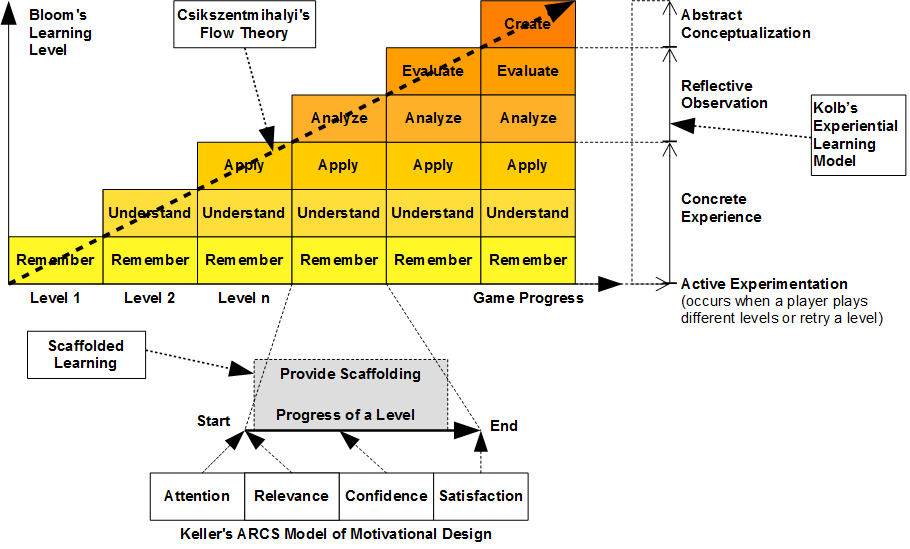
\includegraphics[width=\textwidth]{learning-models}
\caption{Elaborating learning models' contribution to the design of the gamified modeling learning}.
\label{learning-models}
\end{figure}

\begin{figure}[ht]
\centering
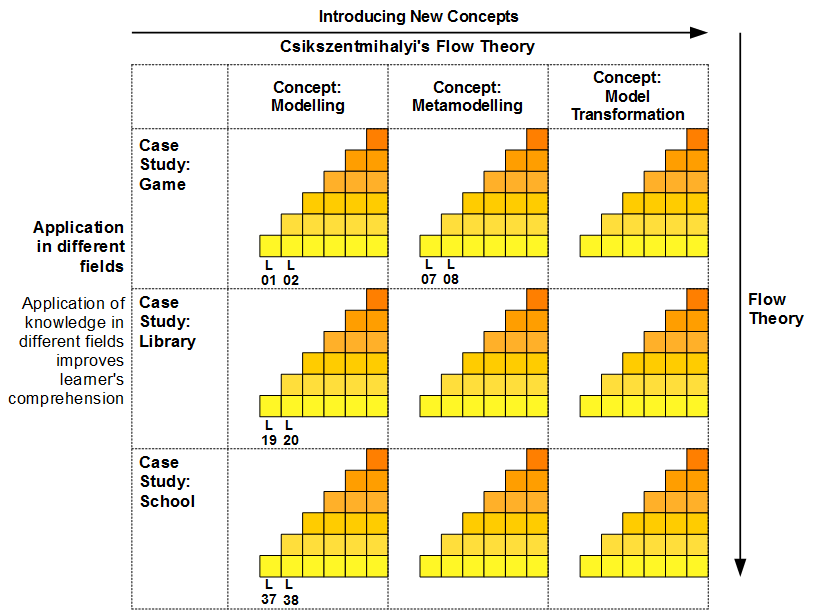
\includegraphics[width=\textwidth]{learning-models2}
\caption{Elaborating learning models' contribution to the design of the gamified modeling learning}.
\label{learning-models2}
\end{figure}

While learners are progressing from levels to levels, they are developing their competence. Thus, difficulty has to be keep balanced with their competence, unless they will get bored. This is the situation where the theory of Flow can be applied (Figure \ref{learning-models}). To control the degree of the difficulty, there are three ways we identified so far related to pedagogical approach: combination of Bloom's activities, introduction of new concepts, and application in different domains. The order of the levels of each of the three ways has to be arranged properly following the theory of Flow. Concepts that are easier are given earlier than the harder ones and the difficulty is increased gradually as learners progress. Likewise, Application in the domains that are more familiar with learners should be given first and gradually shifted to the domains that are most unfamiliar (Figure \ref{learning-models}. Combining these three dimensions--types of activities, concepts, and domains--could give us variety of levels with different degrees of difficulties.

Motivation is an important aspect in the success of learning and we use Keller's ARCS motivational model to address this aspect \cite{keller2010motivational}. we assume that one course of a level is similar to one course of a class meeting, from start to end and between then there are learning activities (Figure \ref{learning-models}). The model provides us in each of it's components--attention, relevance, confidence, satisfaction--a set of predefined techniques to maintain learners' motivation. We could apply this techniques also to maintain learners' motivation along the course of completing a level. As an example, we could use animation to gain learners' attention, explaining the application of the concept being taught in the currently playing level to give relevance, showing their progress in completing a level to maintain their confidence, and giving them reward after finishing a level for reward.
           
We will also apply scaffolding \cite{vygotsky1978mind, wood1976role} to support learners coping challenges (Figure \ref{learning-models}). During the course learners completing a level, scaffolding could be given in several ways: reducing large modelling activities into smaller activity constituents, removing irrelevant activities, providing an almost complete model so they can work on the most relevant activities rather than building the model from scratch, providing help and documentation, and giving some clues of the solutions when they get stuck. Some of this supports will be reduced as players progressing in order to maintain the balance between their increasing competence and difficulty--reducing scaffolding means increasing difficulty.  

We also considering to apply Kolb's experiential learning model, which is a model that agrees knowledge is constructed through experience and based its model on constructivism \cite{kolb2014experiential}. We select Kolb's model since we perceive that playing a level in a game is similar to the learning cycle Kolb proposed; a cycle consists of 4 steps: concrete experience (CE), reflective observation (RO), abstract conceptualisation (AC), and active experimentation (AE). 

We could apply this cycle to frame learners' activities in gaining new knowledge through solving a problem given in a level. For an example, the first time a player plays a new level, at that moment he encounters a concrete experience (CE). Immediately, He attempts to identify and characterise the problem given in that level and recall any knowledge that is relevant to solve the problem (RO). Next, he constructs a solution for the problem that he faces (AC). After constructing the solution, he applies the solution to the problem (AE), experiences the result (CE), and then evaluates whether the solution solve the problem of the level or not (RO). Any gap that appears will update his knowledge. He uses his newly updated knowledge to produce a new solution (AC) that could be applied to the same problem in the same level or different problem in other levels (AE). In case that the player already 'Game Over' and he cannot apply his new solution, AE occurs when he replays the same level or plays another level.

Learning activities in Bloom's taxonomy are also corresponds to the steps in Kolb's learning cycle \cite{murphy2007prior} and both have been applied together to design instructions in different fields \cite{terry1993kolb, howard1996felder, schatzberg2002applying}. Thefor, we argued that both could be applied simultaneously; Bloom's taxonomy provides learning activities while Kolb's model addresses learning cycles in the design of our game. To simplify our work, we summarise the elaboration of design and learning models into a list of requirements (Table \ref{design-learning-models}) that will be used in the design and evaluation activities.

\begin{table}[ht]
\caption{Requirements derived from learning models (section \ref{Elaborating Design and Learning Models}).}
\label{design-learning-models}
\begin{center}
\begin{tabular}{ p{2cm}p{1cm}p{10cm} } 
\hline
Category & Code & Requirements from Learning Models \\
\hline
\multirow{1}{2cm}{Learning Models} 
& RM01 & Design satisfies Bloom's taxonomy. \\
& RM02 & Design suffices Kolb's experiential learning model. \\ 
& RM03 & Design meets Keller's ARCS motivational model. \\
& RM04 & Design fulfils scaffolded learning. \\
& RM05 & Design complies with the theory of Flow. \\      
\hline
\end{tabular}
\end{center}
\end{table}


\section{Game Design}
Gamification has been successfully for a variety of purposes, but there is very little work on software modelling gamification. We wish to assess whether gamification is beneficial for learners of graphical software modelling languages. For each modelling language, we envision the development of a dedicated game containing game elements that will be derived from the Lens of Intrinsic Skill Atoms \cite{deterding2015lens}. The generated game will mimic a graphical modelling tool and at each level, it will require the learner to graphically construct or adapt a model to satisfy a set of requirements and constraints.

\begin{figure}[ht]
\centering
\frame{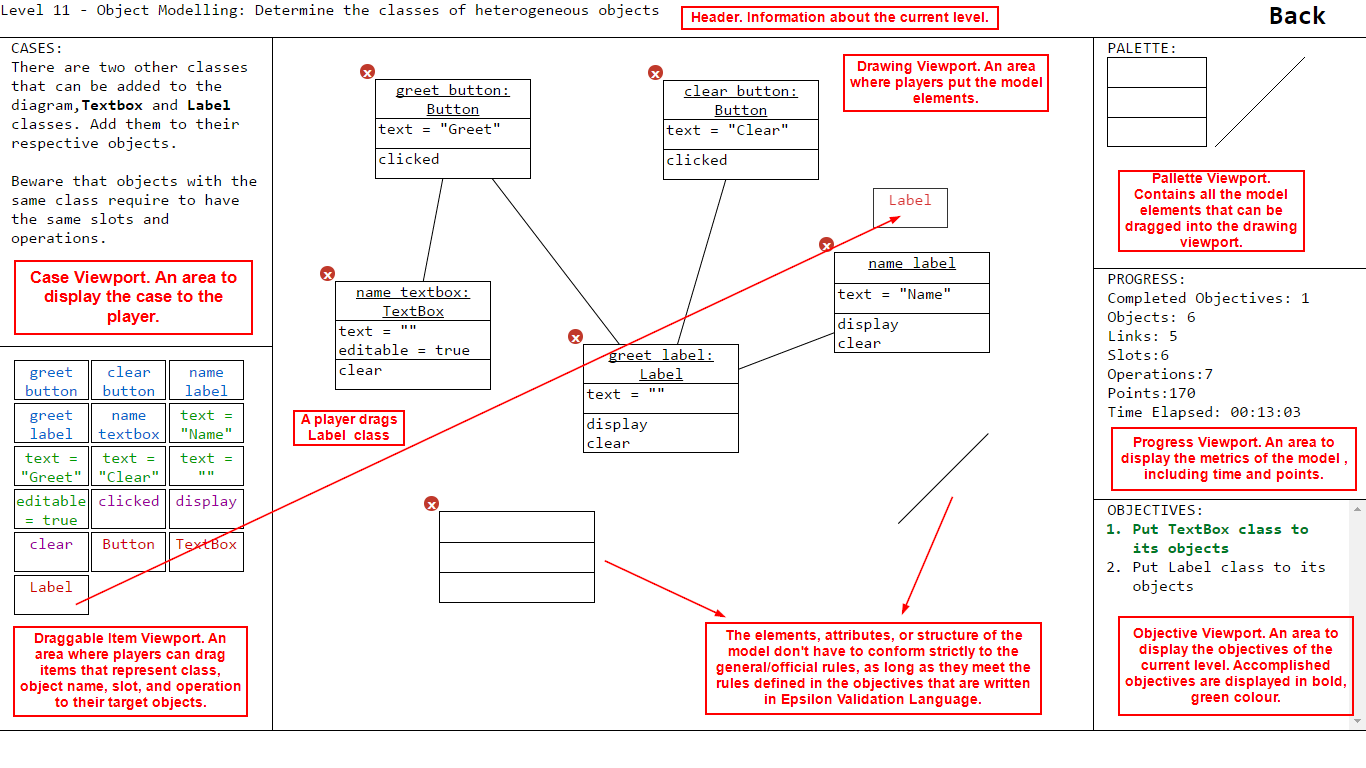
\includegraphics[width=\textwidth]{game-annotated}}
\caption{The display of the generated game.}
\label{fig:001}
\end{figure}

The game will have levels with gradually increasing difficulty as well as variety in its challenges, to expose learners to different kinds of domains, models, and diagrams. Tutorials are planned to be embedded into the game to help learners familiarise themselves with the control system and the flow of the game. 

The game will include interim goals and intrinsic rewards to motivate learners. For software modelling, each type of modelling (e.g. object modelling, collaboration, process) will have several stories. A story will represent a specific case study to introduce learners to problems in specific domains. Every story will consist of several levels, and every level will have one or more objectives that a learner needs to accomplish to complete it. A level may also be a continuation of a previous level, giving the learner a sense of step-by-step progress to complete the domain problems. Each story and level will introduce new concepts and link them with previously introduced concepts.

A real-world problem can be very complex and time-consuming to model. Thus, the extraneous activities that are not relevant to the core concepts that are being taught should be removed. As a result, learners will be more focused on the main concepts. Thus, game elements like bite-sized actions (e.g. drag and drop), limited choices (i.e. only limited items can be dragged), and microflows (i.e. put the right element to its right place) will be implemented to facilitate learners in performing the core activities. Likewise, fuzziness will also be used to provoke learners' creativity since most of the time there is no single correct model for the problem at hand. Attractive design will also be significant to motivate learners to interact with the game. Games should be able to give immediate, glanceable, and actionable feedback to keep learners on track and monitor their progress. Interesting and varied feedback should be designed to appeal to the learners' motives. 

To reduce bias, we plan to experiment with several modelling languages (e.g. BPMN, state-charts, GSN, UML). We also plan to implement these games using web technologies so that they are easily accessible to a wide audience.



\section{Modelling Game Design Framework}
Instead of developing the software modelling games manually, we plan to follow a model-based approach. We will use metamodel annotations, in the spirit of Eugenia \cite{kolovos2015eugenia}, to define the graphical syntaxes of modelling languages and separate models to specify the game elements (levels, objectives, constraints, etc.) of each game. These models will be then consumed by a model-to-text transformation to produce fully-functional language-specific games. Therefore, the framework supports software modelling tutors in the design and customisation of the games at the high level of abstraction and so as to automatically build the game. So far we have implemented a metamodel for specifying game elements (flows, levels, challenges, and objectives) and a supporting Eclipse-based graphical editor (Fig. \ref{fig:002}), and a prototype game (Fig. \ref{fig:001}) for object diagrams. 

\begin{figure}[ht]
\centering
\frame{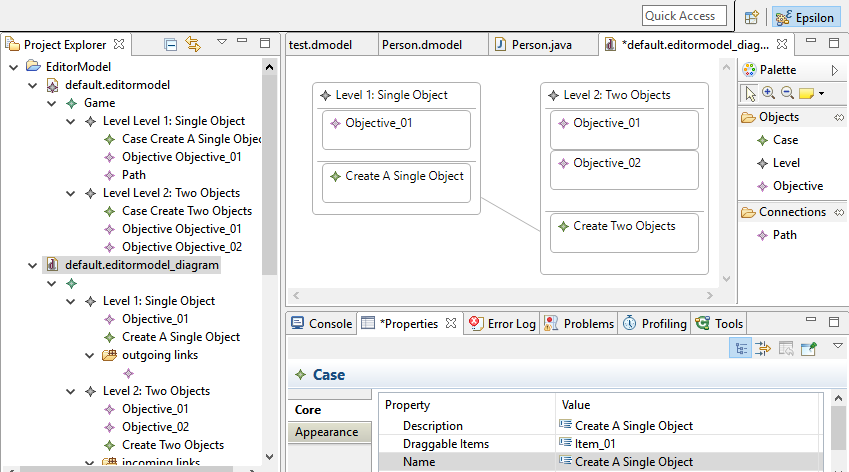
\includegraphics[width=\textwidth]{editor}}
\caption{Graphical editor for the game specification DSL.}
\label{fig:002}
\end{figure}





\addcontentsline{toc}{chapter}{Bibliography}
\bibliographystyle{IEEEtran}
\bibliography{references}

\begin{appendices}

\chapter{Research Plan}
The planned research schedule can be found in Table 1. In three years, this work plans to have five times iteration of Design-Develop-Demonstration-Evaluation, with two of them will be carry out in Indonesia and the rest of them in York.

\begin {table}[ht]
\caption {Research Timetable} 
\end{table}
\begin{figure}[ht]
\centering
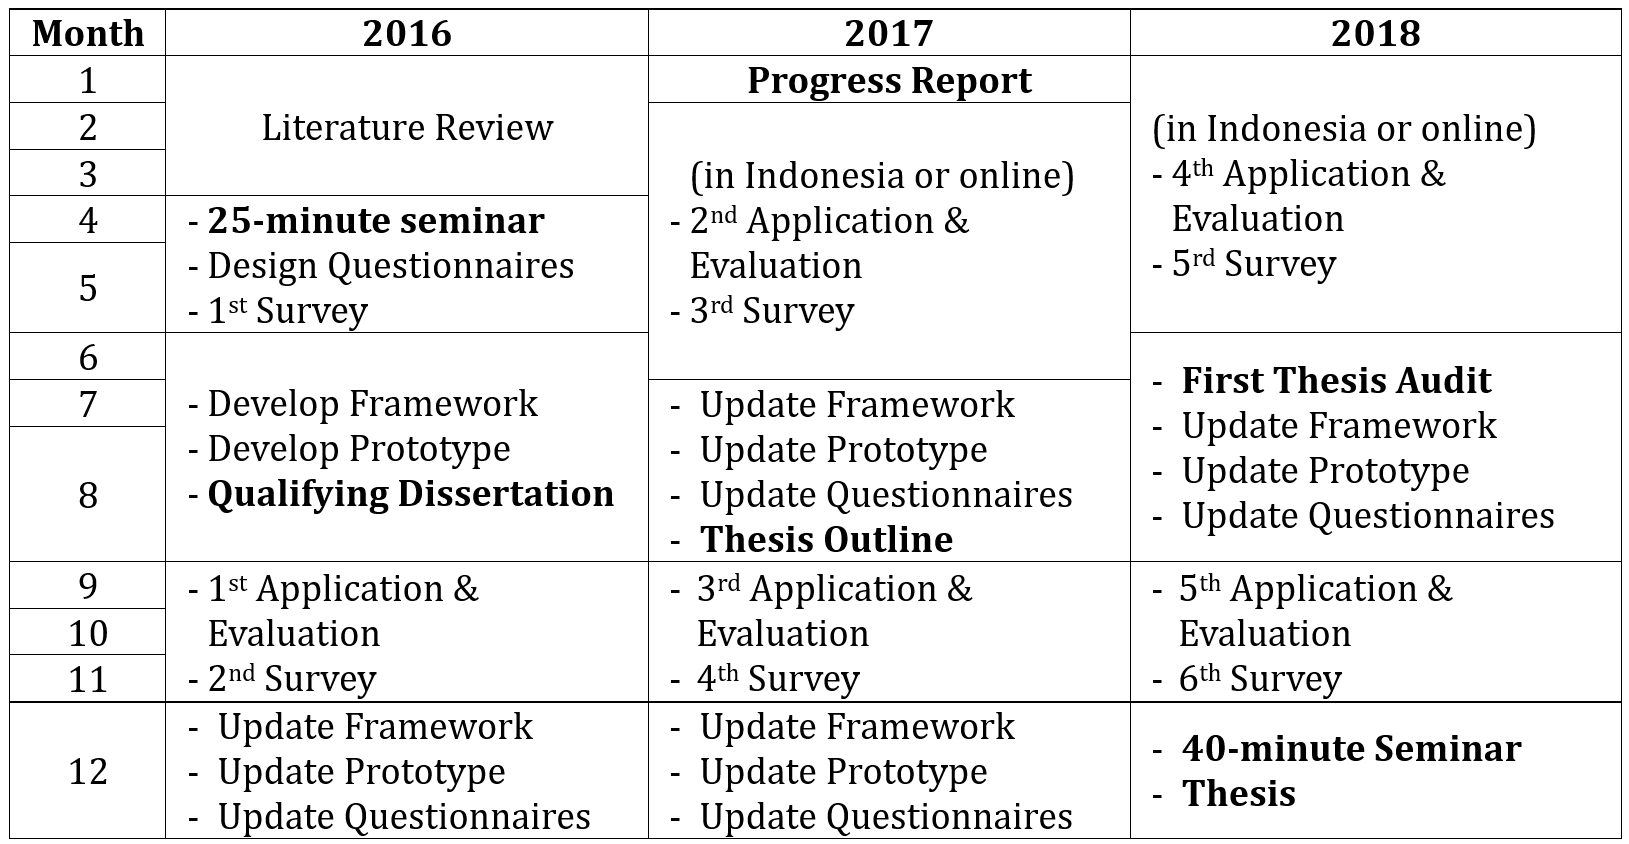
\includegraphics[width=\textwidth]{timetable}
\end{figure}

\chapter{Publications}
This research has been published in the following conferences or journals: 
\begin{enumerate}
 \item A. Yohannis, “Gamification of software modelling,” in the ACM/IEEE 19th International Con-
ference on Model Driven Engineering Languages and Systems (MODELS 2016) Doctoral Sym-
posium. CEUR, 2016 \cite{Yohannis2016}.
\end{enumerate}

\chapter{Preliminary Survey Data}
\label{chap:Preliminary Survey Data}

\begin{enumerate}
\item \textbf{If you think back to the time when you were just about to start the MODE module, what did you think you would find interesting in Model ­Driven Engineering?}
\begin{itemize}
\item Learning what MDE actually is. Had never heard of it so was intrigued.
\item I thought I would be provided with a high level approach to designing and managing software/critical systems.
\item Learning some tools to create auto­models.
\item Learning about ways of statically verifying that code conformed to a formal model, and using this to detect and/or automatically correct bugs learning about ways to automatically modify code based on changes made to a model.
\end{itemize}

\item \textbf{What did you find important in Model­ Driven Engineering?}
\begin{itemize}
\item Domain modelling ­ especially metamodels and the whole concept of abstract syntax. In terms of practicalities, the ability to use models to generate code is the most useful, along with creating DSLs.
\item Trying to learn the specific tools to pass the assessment. Not ideal as I wanted more generic
skillsets in this domain I could apply in my career, instead it was too focused on learning some niche features in Epsilon.
\item abstract thinking ­ validate the models ­ linking the model to real­life.
\item The ability to keep a formal model that the code has been verified to conform to throughout
an entire development process Automatic code generationmodifcation based on a model.
\end{itemize}

\item \textbf{ Why did you decide to take the Model ­Driven Engineering module?}
\begin{itemize}
\item It was compulsory. I had no choice.
\item Compulsory.
\item well, I feel that everything around me has a certain model, therefore, i felt learning about. Model­ Driven will increase my knowledge and experience in work. 
\item It seemed like it would be useful to learn a new approach to software engineering and skills that might be valuable in industry in the future I was interested in generating and transforming code automatically and using a formal model for the structure of code.
\end{itemize}


\item \textbf{ What would motivate you more to learn Model Driven Engineering?}
\begin{itemize}
\item Seeing the MDE approach being used to do something that would otherwise be much more tedious to do using more conventional means.
\item To see the benfit applied in the real world and how organisations have benefited from it. Then how can use these skills and adapt them to my needs.
\item If we link it to real­life examples, explore more other tools.
\item More use of it in industry More use with languages other than java and different types of models such as ones that aren't based on UML/EMF.
\end{itemize}

\item \textbf{ Based on the answers that you’ve provided above (No. 1­4), what were the most basic, core underlying motives or needs that make you commit to learning Model­
Driven Engineering?}

\begin{itemize}
\item The ability to think at a higher level of abstraction and understand the concepts which link together a domain ­ especially, for example, programming languages. 
\item Passing the compulsory paper.
\item see some real­life examples and apply different models to see the differences. 
\item Learning skills which would be valuable in the SE industry in the future Learning something which would help with controlling the complexity of a SE process by making sure that code
conforms to a formally­defined model
\end{itemize}


\item \textbf{ What were the challenges that you found interesting in learning Model­Driven Engineering? Why?}
\begin{itemize}
\item One of the main challenges is in defining the abstract syntax for a DSL along with placing restrictions on its use through a validation language. There's a balance between trying to make the abstract syntax clean and easy to understand and modify vs. preserving the intended semantics.
\item None really, I found the assignment and practicals a tool based grind as opposed to a useful learning opportunity.
\item I felt sometimes that I could not apply all principles in the practicals­ especially on how we think abstract.
\item Working out how to best model a system, which had been defined informally, in EMF and EVL while keeping all its constraints intact and making it easily queryable and transformable was interesting.
\end{itemize}



\item \textbf{How did you manage to overcome these challenges?}
\begin{itemize}
\item By experimenting and going with what makes the most sense. If it's a structural issue with semantics, it's an abstract syntax issue. If it's something more peculiar, it's a validation issue.
\item By grinding through them.
\item I tried to train myself on other examples, but still I could not link my models to real­life example( as real project). 
\item The best way to learn this was from experience which was gained by completing all the practicals.
\end{itemize}


\item \textbf{ What were the hurdles--the non­interesting challenges--that hindered or demotivated you in learning Model­Driven Engineering? Why?}
\begin{itemize}
\item Learning the Eclipse Modelling Framework, MOF etc. wasn't fun. The most fun part was learning and use Emfatic with EGL/EGX and EOL in general. But actually understanding the meta­metamodel and all the ecore stuff seemed pointless. You don't need to understand what EClass, EEnum, EString etc. are. It's just unnecessary detail that's very specific to
Eclipse and not really something that you need to know even if you use Epsilon.
\item The focus on the tool as opposed to the high level concepts and skill sets that would empower me to utilise model driven engineering in the real world.
\item sometime the tool itself, you need to re­track all your changes manually, no right answer or a good explanation why this model is good or bad.
\item Problems using eclipse, the shortcomings of EMF, lack of information available on the internet Eclipse is very large, complex and fragile. EMF/ UML ­style models can be quite restrictive at times when modelling complex relationships, and often requires resorting to EVL. This is annoying because EVL constraints cannot be easily displayed on a diagram and two different languages/systems, EVL and EMF, are being used for similar things. Sometimes two very similar constraints exist where one can be modeled in EMF and the
other can't and so requires EVL. Although there is a lot of very good documentation available about the languages in epsilon there is far less information on the internet about them than what is usually available for popular programming languages and it qould be helpful if there was more.
\end{itemize}

\item \textbf{How did you overcome these hurdles?}
\begin{itemize}
\item By ignoring them; once I realized they served no purpose for developers.
\item Reading up about the tools and grinding through them.
\item Asking questions, reading some examples in the Epsilon website forum.
\item Eclipse sometimes stops working but does this usually does not prevent the completion of tasks as most problems can be fixed by deleting the workspace directory and starting again, it simply wastes a lot of time Things that could not be expressed in EMF were instead expressed using EVL. The required information about epsilon could always be found by
asking classmates and asking lecturers, but this would not be possible if using these languages outside the university
\end{itemize}


\end{enumerate}

\end{appendices}

\end{document}

